\documentclass[11pt]{article}
\usepackage{geometry}                % See geometry.pdf to learn the layout options. There are lots.
\geometry{letterpaper}                   % ... or a4paper or a5paper or ... 
%\geometry{landscape}                % Activate for for rotated page geometry
%\usepackage[parfill]{parskip}    % Activate to begin paragraphs with an empty line rather than an indent
\usepackage{rpmath}
\usepackage{graphicx}
%\usepackage{enumerate}
\usepackage{enumerate}
\usepackage{hyperref}
\usepackage{color}
\usepackage{rotating}

%\usepackage{amssymb}
\usepackage{epstopdf}
\DeclareGraphicsRule{.tif}{png}{.png}{`convert #1 `dirname #1`/`basename #1 .tif`.png}
\catcode`\^^M=10      %  Makes blank lines meaningless to TeX,
                                 % forces useof  \par at paragraph breaks
 
 \usepackage{fancyhdr}
\pagestyle{fancyplain}
\headheight 0 pt
\rhead{}
\chead{}
\lhead{}
\lhead{}
\rfoot{\thepage}
\cfoot{IISc, Mech Eng,  Appl. Dyn. 1:  Homework}
\lfoot{ \today}                                
                                 
\def\tight{ \setlength{\itemsep}{1.5pt}\setlength{\parskip}{0pt}\setlength{\parsep}{0pt}}
 \def\blueref#1{{\color{blue}\bf\ref{#1}}}                           
 \def\bluehref#1#2{\href{#1}{\color{blue}\bf #2}}                           

  \def\vu{\handvec{\bf u}}                                

\title{\vskip -1in \textbf{Homework}\\
EVOLVING DOCUMENT\\
Plaksha:  Dynamics and Simulation\\ \medskip
\normalsize -Andy Ruina
 }
\date{Date of this version:  \today}

\textheight 9 in

\def\Rtensor{\underline{\underline{\mathbf R}}}                            
 \def\Itensor{\underline{\underline{\mathbf I}}}    
 \def\onetensor{\underline{\underline{\mathbf 1}}} 
  \def\ntensor{\underline{\underline{\mathbf n}}} 
   \def\omegatensor{\underline{\underline{\mathbf \Omega}}} 

\begin{document}
\maketitle

\noindent
\href{http://en.wikipedia.org/wiki/Hyperlink}{\color{blue}Hyperlinks look like this.}
 
%%%%%%%%




\section{Problems}




\begin{enumerate} %one for each problem

\item \textbf{} Set up  (define system, draw FBD, write ODEs) a particle problem. Just one particle.
2D or 3D, your choice.
Use a force, or forces that you like (gravity, spring,  air friction). Any example of interest.
Find a numerical solution. Graph it. Animate it.
Try to make an interesting observation.

\par


\item \textbf{3D. Get good at vectors.} Assume that the positions relative to an origin of four random points,  which are randomly located in space are given as $\vrsub{A}, \vrsub{B},\vrsub{C}$ and $\vrsub{D}$. Assume force $\vF$ is given.  For each problem below write a single vector formula (one for each problem) that answers the question. 

\begin{enumerate}[\bf a)]
\item  The points A and B define an infinite line.  So do the points C and D.  Find the distance between these two lines. `The' distance means `the minimum distance', that is the length of the shortest line segment connecting the two lines.  Either write a formula (or sequence of formulas), or write computer code that gives the answer, or both.
\item Same problem as above, but also find the end points of the shortest line segment.
\item Find the volume of the tetrahedron ABCD (you should reason-out and not quote any
formulas for the volume of a tetrahedron, that is, see if you can derive the formula: 'volume = one third base times height').
\item Assume points A, B and C are fixed to a structure.  All three are connected, by massless
rods, to a ball and socket at each end, to point D.  At point D the force $\vF$ is applied.  Find
the tension in bar AD.  Find a formula for the answer, or write computer code to find the answer, or both. The goal is to find a formula for the tension in terms of the positions and the force vector. 

\end{enumerate}

\item {\bf More ODE \& animation practice.}
Take a simple set of ODEs.  Use a set you like,\eg  harmonic oscillator, non-linear pendulum, the Lorentz system (look it up on the internet). Solve this set numerically 3 ways (see below), and understand the accuracy. The goal is that, by the time you hand in the homework, you can write and debug the assignment on your own without looking up anything (outside of trivial syntax things). And you always have a good sense of the accuracy of your solution.
\begin{enumerate}[a.]\tight
\item Method 1:  as simply as possible, without ODE45, and without calling functions or anything like that.  A single function or script file with no function calls (ok, plotting calls are ok). Just write a simple loop that implements Euler's method with your ODE.

\item  With your own Euler solver function.  Your main program should call your Euler solver. Your Euler solver should call a RHS (Right Hand Side) function.

\item With {\tt ODE45}.

\item  Using (b), solve the equations many times with progressively smaller step size, down to the smallest size you
have patience for, and up to the largest size that isn't crazy.  As sensibly as possible,
compare the results and use that comparison to estimate the accuracy of each solution.  You should be able to find a method to estimate the accuracy of a numerical solution even without knowing the exact solution.

\item  Using {\tt ODE45},  solve the equations with various accuracies (use 'reltol' and 'abstol', note \matlab satisfies one or the other, whichever is easiest.  So, if you want an accurate solution you need to make both 'reltol' and 'abstol' small).  Does Matlab do a good job of estimating its own accuracy?  Use suitable plots to make your point.


\end{enumerate}





\item  \textbf{Cross product: geometry vs components.} The geometric definition of cross product is this  $\va \times \vb$ is a vector $\vc$ with magnitude
$|\va||\vb|\sin \theta_{ab}$ that is orthmorogonal to $\va$ and $\vb$ in the direction given by the
right hand rule.   Use this definition to find an alternative geometric definition involving projection 
(namely: project $\vb$ onto the plane that is orthogonal to $\va$; then stretch it by $|\va|$; then rotate it $\pi/2$ around the $\va$ axis). 
Use that definition to  show the distributive rule $\va\times (\vb + \vc) = \va\times\vb + \va\times\vc$.  b) Then use the distributive rule  to find the component formula for cross product, namely that

\[
\va\times\vb =   (a_2b_3-a_3b_2)\uei +  (a_3b_1-a_1b_3)\ueii  + (a_1b_2-a_2b_1)\ueiii.
\]

Note that, this distributive law implies that, for given $va$, $\va\times$ is a linear operator. That
is $va\times\vv$ is a linear function fo $\vv$.  Later in the course we will use this to replace the cross product with a tensor product. 

\textbf{Hint:} You can read about this in, say, the Ruina/Pratap book (box 1.7). 







%%%%
\item{\bf Read up.}  

\begin{itemize}
\item[a.] Read all of the course Teams posts so far, trying out all possible links of interest.
\item[b.] Make sure you thoroughly understand these sections of the Ruina/Pratap pdf book, available from Ruina's www page:  \\
*Chapter 1 (read), \\
*Chapter 2 (skim, only study things you don't know well already, make sure that within a few weeks you know all of this \textit{well}. ), \\
*Chapter 3, \\
*Section 17.1, \\
*Appendix A.

\item[c.] Write the following, if true, if not write that which is true: 

\begin{quotation}\noindent \it ``I have carefully done some of the reading assigned.  That which I don't understand or agree with, I have posted on the course Piazza site.  I haven't yet carefully read  X  {\rm [make appropriate substitutions for X]}''.
\end{quotation}

\end{itemize}



%%%%%%%%%%
\item\textbf{Spring and mass (2D).} One end of of a negligible-mass spring ($k, L_0$) is pinned to the origin, the other to a mass ($m$). There is gravity ($g$).  Initial Conditions (ICs):  The initial position is $\vr_0 = x_0\ui + y_0\uj$, and the initial velocity is $\vv_0= v_{x0}\ui + v_{y0}\uj$. Motion starts at $t=0$ and ends at $t_{\rm end}$.

\begin{enumerate}
\item Find the Equations of Motion (EoM);
\item Assume all parameters and IC's above are given.  
\begin{enumerate}
\item Plot the trajectory of the mass.  
\item Animate the trajectory of the mass.
\end{enumerate}

\item How many ways can you think of checking the numerical solution, find as many as you can, and do the check. The list is started here:
\begin{enumerate}
\item $k=0$, all else arbitrary: The motion is parabolic flight (including falling straight down as a special case) [Why? The system is then just ballistics from freshman physics];
\item $x_0= 0, v_{x0}=0$, all else arbitrary:  The motion stays on the y axis [Why? There is no force in the $x$ direction if the mass is on the $y$ axis. Because the initial velocity has no $x$ component, the mass never leaves the $y$ axis;
\item $g = 0, \vv_0= \vzero$, all else is arbitrary:  The motion stays on a radial line.  And, if the motion does not cross the origin, the motion is that of a harmonic oscillator (sinusoidal oscillations, check by plotting, say $x$ vt $t$.  [Why? Write the EoM  and EoMs in polar coordinates\\ \implies    $m \ddot r  = -k(r - L_0)$ \implies the harmonic oscillator equation, $m \ddot r^*  = -kr^*$, where $r^*\equiv r-L_0$. 
\item $L_0 = 0$, all else is arbitrary:  \underline{\qquad?\qquad}.  [Why?  \underline{\qquad?\qquad}.] Hint, this one special case is problem \ref{HWmasshanging}, below. 
\item \etc
\item \etc
\item \dots



\end{enumerate}

\end{enumerate}




 %%%%
\item {\bf Simple animation of a shape.} Draw a picture of some object (a face, a house, whatever), and make it move around on the screen in a smooth and interesting way.  No distortions. Just motions and rotations.


\item{\bf Simplest dynamics with Polar coordinates.}  This is the simplest dynamics problem, but posed in polar coordinates.  Assume a particle is on a plane with no force on it.  So, you know it moves at constant speed in a constant direction.  


 \begin{enumerate}[a.] 
 \item Write the differential equations
\[
\va = \vzero
\]
 in polar coordinates.   
\item Solve them numerically for various initial conditions.
\item Plot the solution and check that the motion is a straight line at constant
 speed.  
\item Using your numerical result, pick a way to measure how straight the 
 path is, and see how straight a line your polar coordinate solution gives. You should define a quantitative measure of straightness, and then measure it with your solution.
\item  Is the path more straight when you refine the numerical tolerances.
\end{enumerate}
%%%%%%%%%%%%%%%%%%


\item{\bf Canon ball.} \label{HWcanonball} A cannon ball $m$ is launched at angle $\theta$ and
speed $v_0$.  It is acted on by gravity $g$ and a viscous drag with magnitude
$|cv|$.    
\begin{enumerate}  \tight   
       \item Find position vs time analytically.
       \item Find a numerical solution using $\theta = \pi/4$,
           $v_0 = 1\mpers$, $g=1\mperss$, $m= 1 \kg$, $c = 1 \kg/\s$.  
        \item Compare the numeric and analytic solutions.  At $t=2$ how big
          is the error?  How does the error depend on specified tolerances or step sizes?
          \item  Use larger and larger values of $v_0$ and for each trajectory choose
          a time interval so the canon at least gets back to the ground. Plot the trajectories (using equal scale for the $x$ and $y$ axis.  Plot all curves on one plot.  As $v\rightarrow\infty$ what is the eventual shape? [Hint: the answer is simple
          and interesting.]
          
          \item For any given $v_0$ there is a best launch angle $\theta^*$ for
           maximizing the range.  As $v_0\rightarrow\infty$ to what angle does
           $\theta^*$ tend?  Justify your answer as best you can with careful numerics, analytical work, or both.
          
\end{enumerate}
       
     {\par\center{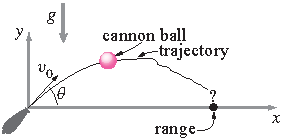
\includegraphics[width = 2.5 in]{HomeworkFigs/cannonball}}\par}  
       
%%%%%%%%%%%%%%%%%%%%%%%%%%%%%%%%%%%%%%%%%%%%%%%%%%%%%%%%%%%%%%%%%%%%%%%%%%%%%%
\item{\bf Mass hanging from spring.} \label{HWmasshanging} 3D. Consider a point mass hanging
from a zero-rest-length linear spring ($\ell_0=0$) in a constant gravitational field.  

\begin{enumerate}\tight
\item Set up equations.  Set up for numerical solution. Plot
2D projection of 3D trajectories.  


\item By playing around with initial conditions, find the
most wild motion you can find (wild means most wiggles, or most complicated). Make one or more revealing plots.
[Hint: Make sure the features you observe are properties of the system and not due to numerical errors. That is, check that the features do not
change when the numerics is refined.]

\item  Using analytical methods justify your answer to part (b).

\end{enumerate} 

 {\par\center{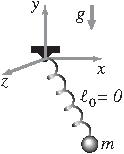
\includegraphics[width = 1.5 in]{HomeworkFigs/mass-spring}}\par}
 
 

%%%%%%%%%%%%%%%%%%%%%%%%%%%%%%%%%%%%
\item{\bf Central force.} \label{HWCentral force}
These two problems are both about central forces. In both cases the only force is central (directed on the particle towards the origin) and only depends on radius:  $\vF = -F(r)\uer$.  The problems are independent, one does not follow from the other.
\begin{enumerate}

\item Find a central force law $F(r)$ so that, comparing  circular orbits of varying radii, the speed  $v$ is independent of radius.  


\item By numerical experiments, and trial and error, try to find a periodic motion that
is \textit{neither} circular nor a straight line, for some central force \textit{besides}
$F= -kr$ or $F= -GmM/r^2$.  a) not with a linear zero-rest length spring;

b) not with inverse-square gravity;
c) not  circular motion; and

d) not straight-line motion.

\begin{enumerate}\tight
\item In your failed searches, before you find a periodic
motion,  do the motions always have
regular patterns or are they sometimes chaotic looking (include some pretty
pictures)?

\item
Puzzle:  If you use a power law, what is the minimum number  loops in one complete periodic orbit (a loop is, say, a relative maximum in the radius)? How does this depend on the exponent in the power law? You probably cannot make progress with this analytically, but you can figure it out with numerical experiments.

\end{enumerate}

\par
[Matlab hint: To do this properly you probably need to guess at a radial force law (most anything will work) and do numerical root finding (\eg {\tt FSOLVE}) to find initial conditions and the period of the orbit.  Once you have your system you can define a function whose input is the  initial conditions and the time of integration and whose output is the difference between the initial state and the final state. You can make this system `square' by assuming that the particle is on the $x$ axis in the initial state.  You want to find that input which makes the output the zero vector.  Pick a central force and search over initial conditions and durations.  Do \textit{not use} {\tt FSOLVE} to search over force laws; do your orbit finding using a given force law. 

\end{enumerate}

 {\par\center{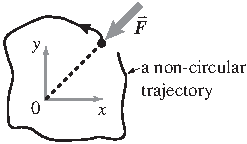
\includegraphics[width = 2.5 in]{HomeworkFigs/centralforce}}\par}

%%%%%%%%%%%%%%%%%


\item{\bf Canon ball 2.} \label{HWcanonball} A cannon ball $m$ is launched at angle $\theta$ and
speed $v_0$.  It is acted on by gravity $g$ and a quadratic drag with magnitude
$|cv^2|$.    
\begin{enumerate} \tight   
   \item Find a numerical solution using $\theta = \pi/4$,
           $v_0 = 1\mpers$, $g=1\mperss$, $m= 1 \kg$.  
    \item Numerically calculate (by integrating $\dot W = P$ along with the state variables) the work done
    by the drag force.  Compare this with the change of the total energy.  Make a plot showing that the
    difference between the two goes to zero as the integration gets more and more accurate.
    
              
       \end{enumerate}

{\par\center{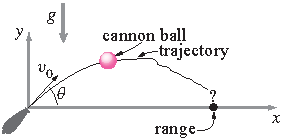
\includegraphics[width = 3 in ]{HomeworkFigs/cannonball}}\par}





\item \textbf{Statics vs Dynamics.} 2D. Equilibrium and dynamics of a point mass $m$ at $\vr_C$. Gravity $g$ points down in the minus $\uj$ direction.  Points A and B are anchored at $\vr_A$ and $\vr_B$. Springs and parallel dashpots connect the mass to A and B. The spring constants are $k_A$ and $k_B$. Their rest lengths are $L_A$ and $L_B$.  Parallel to the springs are dashpots $c_A$ and $c_B$.
The mass also has a drag force proportional to speed through the air $c_d$.   

\par
The dynamic state of the system is described with $z = [ x, y, \dot x, \dot y]'$ and the static state by $z = [ x, y, 0,0]'$.

\begin{enumerate}
\item \textbf{Basic Statics.} Given parameters and an initial guess, find an equilibrium position of this system.  If you have an example you like, post it and people can compare solutions.
\item \textbf{Basic Dynamics.} Given parameters and an initial condition, find the motion.
\item \textbf{All equilibria.}  Given parameters, attempt to find all equilibria.  How many are there? By varying parameters,
what is the most and least number of equilibrium points there can be?
\item \textbf{Stability of equilibrium.} Given an equilibrium point, find it's stability 2 ways: a) With a dynamic simulation near the equilibrium; and b) looking at the eigenvalues of the matrix describing the linearized equations of motion. Compare.
\end{enumerate}
Make appropriate plots, animations and comparisons.  



%%%%%%%%%%%%%%%%%%%%%%%%%%%%%%%%%%%%%%%%%%%%%%%%%%%%%%%%%%%%      
%%%%%%%%%%%%%%%%%%
\item{\bf What means ``rate of change of angular momentum"?}\label{HWwhatmeans}  
Consider a
moving particle P. Consider also a moving  point C  (moving relative to a Newtonian frame $\cal F$ that
has an origin $0$). For which of these definitions of  ${\vH}_{\rm /C}$
Is the following equation of motion true (that is, consistent with $\vF = m\va$)?

\[
\vM_{\rm C}= 
\dot{\vH}_{\rm /C}
\]

In each case say whether the definition works
 i) in general, or  ii) for some special cases (that you name) concerning the motions
of P and C.  

\begin{enumerate}\tight
\item{$\vH_{/C} = \vr_{\rm P/C'}\times \vv_{\rm P/0}m$, \\ where C' is a
point fixed in $\cal F$ that instantaneously coincides with C.  }


\item{$\vH_{/C} = \vr_{\rm P/C}\times \vv_{\rm P/0}m$.  }


\item{$\vH_{/C} = \vr_{\rm P/C}\times \vv_{\rm P/C}m$.  }

\end{enumerate}

That is, for  each possible definition of  ${\vH}_{\rm /C}$ you need to
calculate  $\dot{\vH}_{\rm /C}$ by differentiation and see if and when
you get $\dot{\vH}_{\rm /C}=\vrsub{P/C}\times m\vasub{P/\cal F}$.

{\par\center{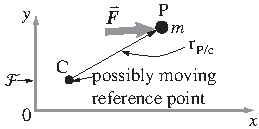
\includegraphics[width = 2.5 in]{HomeworkFigs/Def-of-H}}\par}

\item{\bf Potential Energy}
For each of the force fields below, find the associated potential energy function.
All of them are 3D.  In some cases the energy is associated with the positions of
two particles.  Any free constant can be set to a convenient value (like zero). The answers are
easy, it sometimes takes careful multi-variable calculus to find or check them.

\begin{enumerate}

\item  Constant force $\vF = -mg\uj$.  (Ans: $E_p = mgy$)
\item  Zero-rest-length spring, one end at origin $\vF = -kr\uer= - k\vr$.  (Ans: $E_p = kr^2/2$)
\item  Spring, one end at origin $\vF = -k(\ell - \ell_0)\uer$.  (Ans: $E_p = k(\ell-\ell_0)^2/2$)
\item  Inverse square central force $\vF = -C \vr/r^3$.  (Ans: $E_p = -C/r$)
\item  Central force, depending on $r$, $\vF = -f(r)\uer$.  (Ans: $\int_{r_0}^r f(r')\, dr'$, with
$r_0$ chosen so the integral is not divergent)
\item  Spring between two points.  (Ans: $E_p = k (\ell_{12} - \ell_0)^2/2$)
\item  Inverse square attraction between two points.   (Ans: $E_p = -C/\ell_{12}$)
\item  Constant force $\vF = - C\ul$.  (Ans: $E_p =C \vr\cdot \ul$)
\item  Force in $x$ direction only depending on $x$,  $\vF = -f(x)\ui$.  (Ans: $\int_{x_0}^x f(x')\, dx'$, with $x_0$ chosen so the integral is not divergent)
\end{enumerate}
%%%%%%%%%%%%%%%%




\item{\bf Mechanics of two or more particles}\label{HWtwoormore}  

\begin{enumerate}\tight
\item For two unequal particles with mass $m_1$ and $m_2$ what is the period of circular motion
if the distance between the particles is $d$ and the only force is the force between them is from classical inverse-square Newtonian gravity,
$F= Gm_1m_2/r^2$?  
\item Pick numbers for $G,m_1,m_2$ and $r$ and, using appropriate initial conditions, test
your analytical result with a numerical simulation.  Make any plots needed to make the agreement of
your numerical and analytical results convincing.

\item For three equal particles, $m_1=m_2=m_3=1$ and $G=10$ what is the angular
speed for circular motion on a circle with diameter of $d=3$?

\item Check your result for three particles with a numerical simulation, as you did for 2 particles, above.
\end{enumerate}

{\par\center{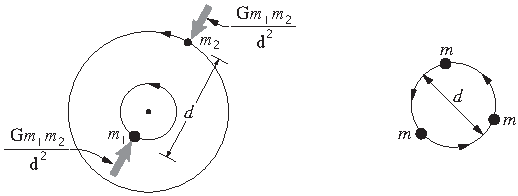
\includegraphics[width = 2.5 in]{HomeworkFigs/two-particles}}\par}




%%%%%%%%%%%%%%%%
 \item\textbf{Montgomery's eight.} \label{HWmontgomery} (From Ruina/Pratap).

Three equal masses, say $m=1$, are attracted by an inverse-square gravity law
with $G=1$. That is, each mass is attracted to the other by 
$F = Gm_1m_2/r^2$ where $r$ is the distance between them. 
 Use these unusual and special initial positions: 

\begin{eqnarray*}
(x1,y1) &=& (-0.97000436, 0.24308753)\\
 (x2,y2) &=& (-x1, -y1)\\
  (x3,y3)& =& (0,0)
\end{eqnarray*}
 and 
initial velocities 
 \begin{eqnarray*}
 (vx3,vy3)& =& (0.93240737, 0.86473146)\\
 (vx1,vy1) &=& -(vx3, vy3)/2\\
 (vx2, vy2) &=&  -(vx3, vy3)/2.
  \end{eqnarray*}
For each of the problems below show accurate computer plots and explain
any curiosities.
\begin{enumerate}\tight
\item 
Use computer integration to find and  plot the motions of the particles.
Plot each with a different color.  Run the program for 2.1 time units.


\item Same as above, but run for 10 time units.


\item Same as above, but change the initial conditions slightly.


\item Same as above, but change the initial conditions more and run for a much longer time.



{\par\center{\includegraphics[width = 2.0 in]{HomeworkFigs/montgomery-8}}\par}

{\small [Aside:  This was discovered  by both Richard Montgomery (Santa Cruz Math department) and also
 by ex-Cornell Physics PhD student Chris Moore (now at Santa Fe Institute), independently. And, I know both of them, independently.]}
\end{enumerate}




 %%%%%%%%%%%%%%%%%%
  \item\textbf{Konig's Theorem} \label{HWKonig} The total kinetic energy of a system of
  particles is
  
  \[
  \KE = \frac{1}{2} \sum m_i v_i^2.
  \]
 
 \begin{enumerate}\tight
\item  Derive an expression of this form
 
 \[
  \KE =  \frac{1}{2}\mtot v_G^2   +  ...  \textrm{you fill in the rest} ... .
  \]
 
 \item  Is it always true that
 
 \[
\left( \sum \vF^{ext}\right)\cdot \vvsub{G} = \frac{d}{dt} \left( \frac{1}{2}\mtot v_G^2\right)  ?
 \]
 
 Defend your answer with unassailable clear reasoning (that is, a proof or a counter-example).
 
 \item  Is it always true that the power of internal forces is equal to the rate of change of the quantity you filled in part (a) above (just the second half of the full expression)?  Provide a proof or a counter-example. (A good solution is expected from those
 in 5730).
 
 {\par\center{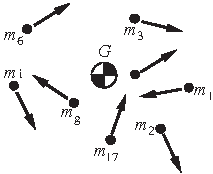
\includegraphics[width = 2.0 in]{HomeworkFigs/Konig}}\par}

 \end{enumerate}
 


 %%%%%%%%%%%%%%%%%%%%%%%%%%%%%%%%%%%%%%%%%%%%%%%%%%%%%%%%%%%%%%%%%%%%%%%%%%%%%%
\item{\bf What means ``rate of change of angular momentum" for a SYSTEM of particles?}\label{HWwhatmeans2}  
You should master problem \ref{HWwhatmeans}  before looking at this problem.  Consider a system of moving particles with moving center of mass at G. Consider also a moving  point C  (moving relative to a Newtonian frame $\cal F$ that
has an origin $0$). For which of these definitions of  ${\vH}_{\rm /C}$
Is the following equation of motion true (that is, consistent with $\vF = m\va$)?

\[
\vM_{\rm C}= 
\dot{\vH}_{\rm /C}
\]

In each case say whether the definition works
 i) in general, or  ii) for some special cases (that you name) concerning the motions
of P and C.  

\begin{enumerate}\tight
\item{$\vH_{/C} = \sum\vr_{\rm i/C'}\times \vv_{\rm i/C'}m_i$, \\ where C' is a
point fixed in $\cal F$ that instantaneously coincides with C.  }\\
(Hint: this definition is good one, always!)


\item{$\vH_{/C} = \sum\vr_{\rm i/C}\times \vv_{\rm  i/0}m_i$.  }\\
(This strange definition is used in the classic, but in this case odd,  Dynamics book by Housner and Hudson.)


\item{$\vH_{/C} =\sum \vr_{i/C}\times \vv_{i/C}m_i$.  }\\
(Hint: this is the most important candidate definition, but it's only good for special
kinds of C, namely:  C = COM,  C is fixed and ...?)

\end{enumerate}

That is, for  each possible definition of  ${\vH}_{\rm /C}$ you need to
calculate  $\dot{\vH}_{\rm /C}$ by differentiation and see if and when
you get $\sum\vrsub{i/C}\times \vasub{i/0}m_i$.   If you are short for time just consider cases (a) and (c)
and note their agreement  if C is stationary or if C=G. Students in 5730 are expected to do a competent clear job of all three parts.

{\par\center{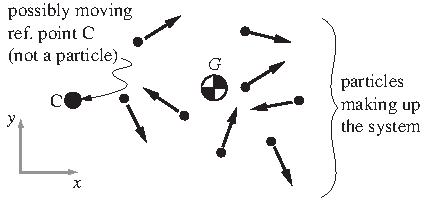
\includegraphics[width = 3 in]{HomeworkFigs/Def-of-H-many}}\par}


  %%%%%%%%%%%%%%%%%%
  \item\textbf{Two masses} \label{HWtwomasses} This problem has 3 independent educational goals:
  \begin{enumerate}\tight

 \item  Motivate the use of kinematic constraints.

  \item Introduce the simplest of a class of vibrations problems which you should master. At this point, it is this aspect: mastery of derivation of the equations of motion.  You should check that you can reproduce the lecture example with \textit{no} sign errors without looking up anything.
  
  \item Development of critical exploration using analytical and numerical methods.
   
  \end{enumerate}
  
  Two masses $m_1$ and $m_2$ are constrained to move frictionlessly on the $x$ axis.  Initially they are stationary
  at positions $x_1(0)=0$ and $x_2(0)= \ell_0$.  They are connected with a linear spring with constant
  $k$ and rest length $\ell_0$.  A rightwards force is applied to the second mass.  It is a step, or `\bluehref{http://en.wikipedia.org/wiki/Heaviside_step_function}{Heaviside}' function
  
  \[
  F(t) = F_0 H(t) = 
  \begin{cases}
   0& \mbox{if } t<0\\
  F_0&\mbox{if } t\ge 0 
  \end{cases}
  \]
  
    \begin{enumerate}\tight
  \item Write code to calculate, plot and (optionally) animate the motions for arbitrary values of the
  given constants.
  
  \item  Within numerical precision, should your numerical solution always have the property that 
 $ F= (m_1+m_2)a_G$  where $x_G = (x_1m_1 + x_2m_2)/(m_1 + m_2)$? (As always in this course, ``yes or no''
 questions are not multiple choice, but need justification that another student, one who got the opposite answer as you, would find convincing. )
 \item Use your numerics to demonstrate  that if $k$ is large the motion (displacement relative to its starting position) of \textit{each} mass is, for time scales large compared to the oscillations,  close to the center of mass motion.
 
 \item  5730 only:  Using analytic arguments, perhaps inspired by and  buttressed with numerical examples, make the following
 statement as precise as possible: \medskip 
 \par

  \textit{\qquad For high values of $k$ the system nearly behaves like a single mass.} 
 \par
  \medskip
  
   Of course, in detail, the system has 2 degrees of freedom (DOF).  So you are looking for a way to
 measure the extent to which the system acts like it has 1 DOF, and in which conditions (for which extreme values of parameters and times) the system
 is close to 1 DOF by that measure. There is not a simple single unique answer to this question.
 
 
   \end{enumerate}

 
  {\par\center{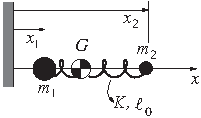
\includegraphics[width = 2.5 in]{HomeworkFigs/Two-DoF-spring}}\par}




%%%%%%%%%%%%%%%%%%%%% 
\item\textbf{Two masses constrained} \label{HWtwomassesconstrained} This is an elaboration of the
  problem above, replacing the spring with a rigid rod.  As per lecture, set up the DAEs and 
  solve them using Matlab using numbers of your choice. Use a forcing $F$ that varies sinusoidally in time.
    Note the increasing error (as time progresses) in the satisfaction of the constraint.
  Compare this solution with the the method from the problem above (where you use some very large value of $k$). Which  one is is faster to compute on the computer? Which is more accurate in predicting COM motion? (Again, as always, justify your answer so someone who disagrees would be convinced.) Try putting in initial conditions in which
  the masses have unequal initial velocity; explain as best you can the result you get, and why.
  
  
 
   {\par\center{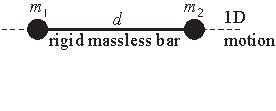
\includegraphics[width = 2.5 in]{HomeworkFigs/Bar-two-masses}}\par} 
  
 %%%%%%%%%%%%%%%%%%%%%%% 
\item{\bf Simple pendulum.} \label{HWsimplependulum} Derive the simple
pendulum equation $\ddot\theta +{g\over\ell}\sin\theta=0$ as many ways as you can
without looking anything up in books.  For example, in all cases using polar coordinates,
\begin{enumerate}\tight
\item linear momentum and manipulate the equations to eliminate constraint force
\item linear momentum, dot with $\ueth$
\item linear momentum, cross with $\vr$
\item angular momentum
\item conservation of energy
\item power balance
\item Lagrange equations (if you know them already, not if you don't).
\end{enumerate}
%%%%%%%%%%%%%%%%%%%%%%%%%%



\item{\bf Pendulum numerics.} \label{HWpendulumnumerics}
Set up the pendulum in cartesian coordinates. Express the constant
length constraint as a set of linear equations restricting the acceleration.
Solve these (3 2nd order) DAE equations with numerical integration and initial conditions and parameters of your choosing. No polar coordinates allowed.  Quantitatively compare your solution with a solution of the simple pendulum equations (For the comparison you need to either compute $x$ from $\theta$ or \textit{vice versa}.
Integrate for a long enough time so you can detect drift away from satisfying the kinematic constraint.
%%%%%%%%%%%%%%%%%%%%%%%%%%%%%%%




\item{\bf Pendulum with an awkward parameterization} \label{HWbadparam}
By any means you like, for a simple pendulum find the equations of motion  using $y$ (horizontal position) as your parameterization
of the configuration.  That is, find a 2nd order differential equation determining $\ddot y$ in terms of $y$, $\dot y$ and physical parameters ($g,m,\ell$).   Using numerics, quantitatively compare the solution of this ODE with a solution of the simple pendulum equations (Note, you can assume the pendulum is hanging down, hence $x>0$.  This problem is
different from the DAE problem above in that you should obtain a single 2nd order ODE, not a set of 3 equations.  
  
  
  %%%%%%%%%
  \item{\bf 2D Dumbell.} \label{HW2Ddumbbell} Two equal masses $m=1$ are constrained by a rod to be a distance
  $\ell=1$ apart.  There are no non-negligible forces, except from the constraint. At $t=0$ they have equal and opposite velocities ($v=1$) perpendicular to the rod.  Use a set of 5 DAEs ($\vF=m\va$ \& the constraint equation $(x_2-x_1)^2 + (y_2-y_1)^2 = \ell^2$ with numerical integration to find the
  subsequent motion.  Use plots and/or animation to help debug your code.  Using what you know about  systems of particles (\eg momentum, angular momentum, constraint equation, energy) quantify as many different numerical errors   as you can.
  
  

  %%%%%%%%%%%%%%%%%%%%
  \item{\bf Rotation with zero angular momentum.}\label{HWwhatmeans2}
  
  This is a concrete example showing that a system can rotate while having zero angular momentum
  at all times.  If you don't like this example, or want to do a different one for any reason, any substitution
  is fine.  But it needs to be backed by a clear (numerical is fine) calculation.
  \par
  
  Consider a massless rigid plate in space.  On this plate are marked $x$ and $y$ axes.   
There are 4 equal masses attached to the plate.    Two of them are welded (glued, fixed) to the plate
on the $y$ axis at $y=\pm 2$.  Two of them are forced, by massless machinery that rides on the plate,
to move in a circle  with radius $r=1$ centered at $ x = \pm 2$, and starting at $x= \pm 3$,  respectively.   They move such that
the line connecting them goes through the origin at all times.  The right mass moves according to this
equation, using polar coordinates centered at $y=0, x=2$:

\[
r=1,  \qquad\qquad \theta =\left(1-\cos(t) \right)\pi   \quad \mbox{for} \quad \mbox  0\le t \le \pi.
\]
  
  That is, the mass goes around the circle once in a nice smooth motion.
  
  The other mass moves accordingly (same motion, reflected through the origin).  
  
  
  \par
  
  Use conservation of angular momentum for the system to find
  the net rotation $\phi$ of the masses on the $y$ axis at the end of one rotation of the $x-$ axis masses.
  Numerical integration is fine. [Hint:  The equation  $\vH_{/0}=\vzero$ tells you $\dot\phi(t)$.]  
  
  {\par\center{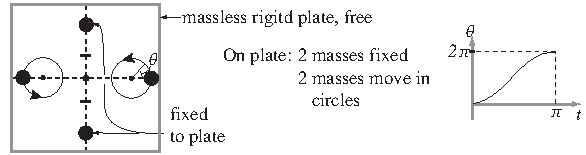
\includegraphics[width = 4 in]{HomeworkFigs/Rot-with-no-H}}\par}
  

  %%%%%%%
\item {\bf Canonball.} (Continuation of problem 10) A cannon fires a projectile that experiences gravity and quadratic drag $F_D = c_Dv^2$). Cannonball mass  $m = 1\kg$, acceleration due to gravity $g=10\mperss$, and drag coefficient is $c_D = 0.5\kg/\m$. 


  
\begin{enumerate}[i.]
\item Find a trajectory (using whichever numerical tool you choose, but don't just guess!) so that the projectile hits the ground at $x = 2\m$ given using a launch speed of $v_0=10\mpers$. Find the launch  angle and a plot of the trajectory.
\item 	Imagine you want an efficient cannon that can hit a point at least $2\m$ away with the minimum possible launch speed. Find  the angle and launch velocity that achieve this. 
\end{enumerate}


  
  %%%%%%%
\item Reconsider the Montgomery 8  problem again (3 point masses mutually attracted by gravity) using $m_i = G = 1$.  Find a periodic solution by optimizing both the initial conditions and simulation time so that the error between initial and final state (positions and velocities) goes to 0. Afterwards simulate for  5+ periods to demonstrate that your solution is periodic.

The following initial conditions are a reasonable guess:\\ \\
\textbf{Mass 1:}
X1=-0.755;
Y1=0.355;
Vx1=0.9955;
Vy1=0.07855;\\ \\

\textbf{Mass 2:}
X2=1.155;
Y2=-0.0755;
Vx2=0.1055;
Vy2=0.4755;\\ \\

\textbf{Mass 3:}
X3=-0.4055;
Y3=-0.3055;
Vx3=-1.1055;
Vy3=-0.5355; \\ \\

A good initial  guess for the period is  8 (8 time units) .

Hint: You'll be most successful if you bound your search near to these values. If you don't use variable bounds (e.g. in FMINCON), you'll probably find the trivial solution where everything equals 0. If you want to go on with this problem, you can try it again  using Matlab's BVP4C command (which is said to do this particular problem more elegantly). 
  
  
\par
Etra:  See if you can find any other periodic solutions of the 3-body problem.
  
  %%%%%%%%%%%%%%%%%



%%%%
\item{\bf Inverted pendulum with shaking base.}  A uniform stick with length $\ell$ is
connected to a hinge at its lower end.  That hinge is shaking up and down with a specified
acceleration $a(t)$ (could be a specified position, differentiated twice).  

\begin{enumerate}
\item Find the equations of motion.
\item Simulate the motion to show that the pendulum can be stable when upright.
[Hint: Use an oscillating base with a small displacement amplitude ($\delta\ll \ell$) and a
 big enough frequency ($a\gg g$).]
 \item Do again with DAEs, and show that your results quantitatively agree.


\end{enumerate}


 %%%%%%%%%%%%%%%%%
%%%%%%%%%%%%%%%%%%%%%%%
\item {\bf Bead on parabolic wire }\label{HWbeadonwire}
For a frictionless point-mass bead sliding on a rigid wire on the curve
$y=cx^2$ with gravity in the $-y$ direction, find the equation of motion. 

\begin{enumerate}\tight

\item Derive the equations of motion using  the $x$ axis as the minimal (generalized)
coordinate.   Use Newton's laws.

%\item Derive the equations of motion using Newton's laws. First
%write $\vF = m\va$ with an unknown constraint force orthogonal to the wire.
%Then dot both sides with a vector tangent to the wire. You should get the
%same answer as for part (a) with a very similar amount of algebra.
%
%\item Find the frequency of small vibrations (find a formula for this in terms
%of some or all of  $m$,$g$ and $c$.

\end{enumerate}

 %%%%%%%%%%%%%%%%%

    %%%%%%%%%%%%%%%%%%%%%%%%%%%%%%%%%%%%%%%%%%%%%%%%%%%%%%%%%%%%%%%%%%%%%%%%%%%%%%
\item{\bf Double pendulum. 2D.}\label{HWdoublependulum} A double pendulum is made
with two bars.  Hinges are at the origin 0 and the elbow E.    $g=1$. Neglect all friction and assume there are no joint motors.

\begin{enumerate}\tight
\item Set up and numerically solve (there is no analytic solution) to the  governing equations that you find using  AMB. You may refer to lecture notes, but you should be able to do it on your own by the time you hand in the work.   Assume that at $t=0$
the upper arm is horizontal, sticking to the right, and the fore-arm is vertical up (like looking from the
front at a driver using hand signals to signal a right turn).  Integrate until $t=30$.  Draw the (crazy) trajectory of
the end of the forearm.  For definiteness (and so you can check solutions against each other) use  parameters corresponding to equal-length uniform bars with length 1 and use $g=1$.



\item Solve again by DAEs equations.   By comparing numerical solutions, show that
the governing equations are the same as those obtained using AMB. 

\item  And again with Lagrange equations, and compare again.

\item  Animate your solution.  Put your solution in a folder.  Name the folder:  YOURNAME-Double.   In the folder have a function called ROOT (and other
well-commented Matlab files).  Running ROOT should give an animation within 30s.  Zip the folder.  Call the zipped file YOURNAME-Double.    Have that ready to send to your TA.

\item  Extra things you can do:

\begin{enumerate}
\item  Explore various options for setting up the ODEs. For example:  cut and paste from symbolic toolbox, Jacobian, EquationsToMatrix.  When using DAEs: extract the minimal coordinate angular accelerations vs consider the motion of the independent rigid objects (6 DoF system). 
\item  Use various checks: Compare methods by subtracting one result from the other; if applicable, check energy conservation or angular momentum conservation  by plotting the value, subtracting the initial value.
\item Think of as many special cases as you can where you know something about the solution without doing a numerical solution.
\item make your animation and plotting and nice as you can.
\item \etc


\end{enumerate}

\end{enumerate}





%%%%%%%%%%%%%%%%%%%%%%%%%%%%%%%%%%%%%%%%%%%%%%%%%%%%%%%%%%%%%%%%%%%%%%%%%%%%%%
  \item{\bf Braking stability}\label{HWbrakingstability} 2D, looking down.  Consider the steering stability of a car going straight ahead with either the front brakes locked
or the rear brakes locked.  The steering is locked and straight ahead.  For simplicity
assume that the center of mass is at ground height between the front
and back wheels.  Assume that the locked wheels act the same as a single
dragging point on the centerline of the car, midway between the wheels. 

\begin{enumerate}
\item{Develop the equations of motion.  }


\item{Set them up for computer solution. Note:  ODE45 is generally unhappy when the car comes to a stop (because of a divide by $v$ in your code).  One way to avoid this is by using the `events' option to stop the calculation when the speed gets down to some very small number. } 


\item{For some reasonable parameters and initial conditions
find the motion and make informative plots that answer the question
about steering stability. Note, in this problem where there is no
steady state solution you have to make up a reasonable definition
of steering stability.} 


\item{See what analytical results you can get about the
steering stability (as dependent on the car geometry, mass distribution,
the coefficient of friction and the car speed).
As much as  you have time and interest, illustrate your results with graphs and animations of 
numerical integrations.}

\item \textbf{Things to think about.} 

\begin{enumerate}
\item Check that your governing equations reduce to the lecture (ideal, no friction) equations when the friction is zero.
\item Check special cases of the  numerical solutions with solutions you know other ways.  A challenge is to think of as many of these as you can (even if you don't check all of them).   That is, for some special parameter values and/or initial
conditions you know features of the solution (examples: 
\begin{enumerate}
\item No friction means energy is conserved;
\item With friction and no initial rotation  slowing is with constant acceleration, 
\item \etc  
\end{enumerate}


\end{enumerate}

\end{enumerate}

%%%%%%%%%%%%%%%%%%%%%%%
\item {\bf Bead on parabolic wire, Lagrange Equations }\label{HWbeadonwire}
For a frictionless point-mass bead sliding on a rigid wire on the curve
$y=cx^2$ with gravity in the $-y$ direction, find the equation of motion. 

\begin{enumerate}\tight

\item Derive the equations of motion using  the $x$ axis as the generalized
coordinate.  Check that this agrees with the Newton-Euler approach.

\item A curve in the $xy$ plane is described by the following equation:

\[
y = cs^2,
\]

where $s$ is arc-length along the curve $y = cs^2$, starting at $x=y=0$ 
($x$ is only defined implicitly on this curve, using the equation $ds = \sqrt{(dx)^2 + (dy)^2}$.  A bead slides
on that wire with gravity.  Use Lagrange equations to find the EoM. [Hint: this
is a really easy problem]. \\  Extra credit:

\begin{enumerate}[\bf i)]

\item  draw the curve (probably requires 
numerical integration or ODE solution),

\item  find a more normal
description for the curve (e.g., a parametric equation), [Hint:  It is a famous curve,  with a special name and
all.] 

\end{enumerate}

%\item Derive the equations of motion using Newton's laws. First
%write $\vF = m\va$ with an unknown constraint force orthogonal to the wire.
%Then dot both sides with a vector tangent to the wire. You should get the
%same answer as for part (a) with a very similar amount of algebra.
%
%\item Find the frequency of small vibrations (find a formula for this in terms
%of some or all of  $m$,$g$ and $c$.

\end{enumerate}


 %%%%%%%%%%%%%%%%%%%%%%%%%%%%%%%%%%%%%%%%%%%%%%%%%%%%%%%%%%%%%%%%%%%%%%%%%%%%%%

\item{\bf Mass in slot on turntable.}\label{HWmassinslot} A rigid turntable ($m_t,I_t$) is free to rotate about a hinge at it's center. It has in it a straight frictionless slot that passes a distance $d$ from it's center.  A mass $m_s$ slides in the slot. For minimal coordinates use rotation of the disk
$\theta$ from the position in which the slot is horizontal and below the disk center, and the distance $s$ the mass is from the point where the slot is closest to the center of the disk.  


{\par\center{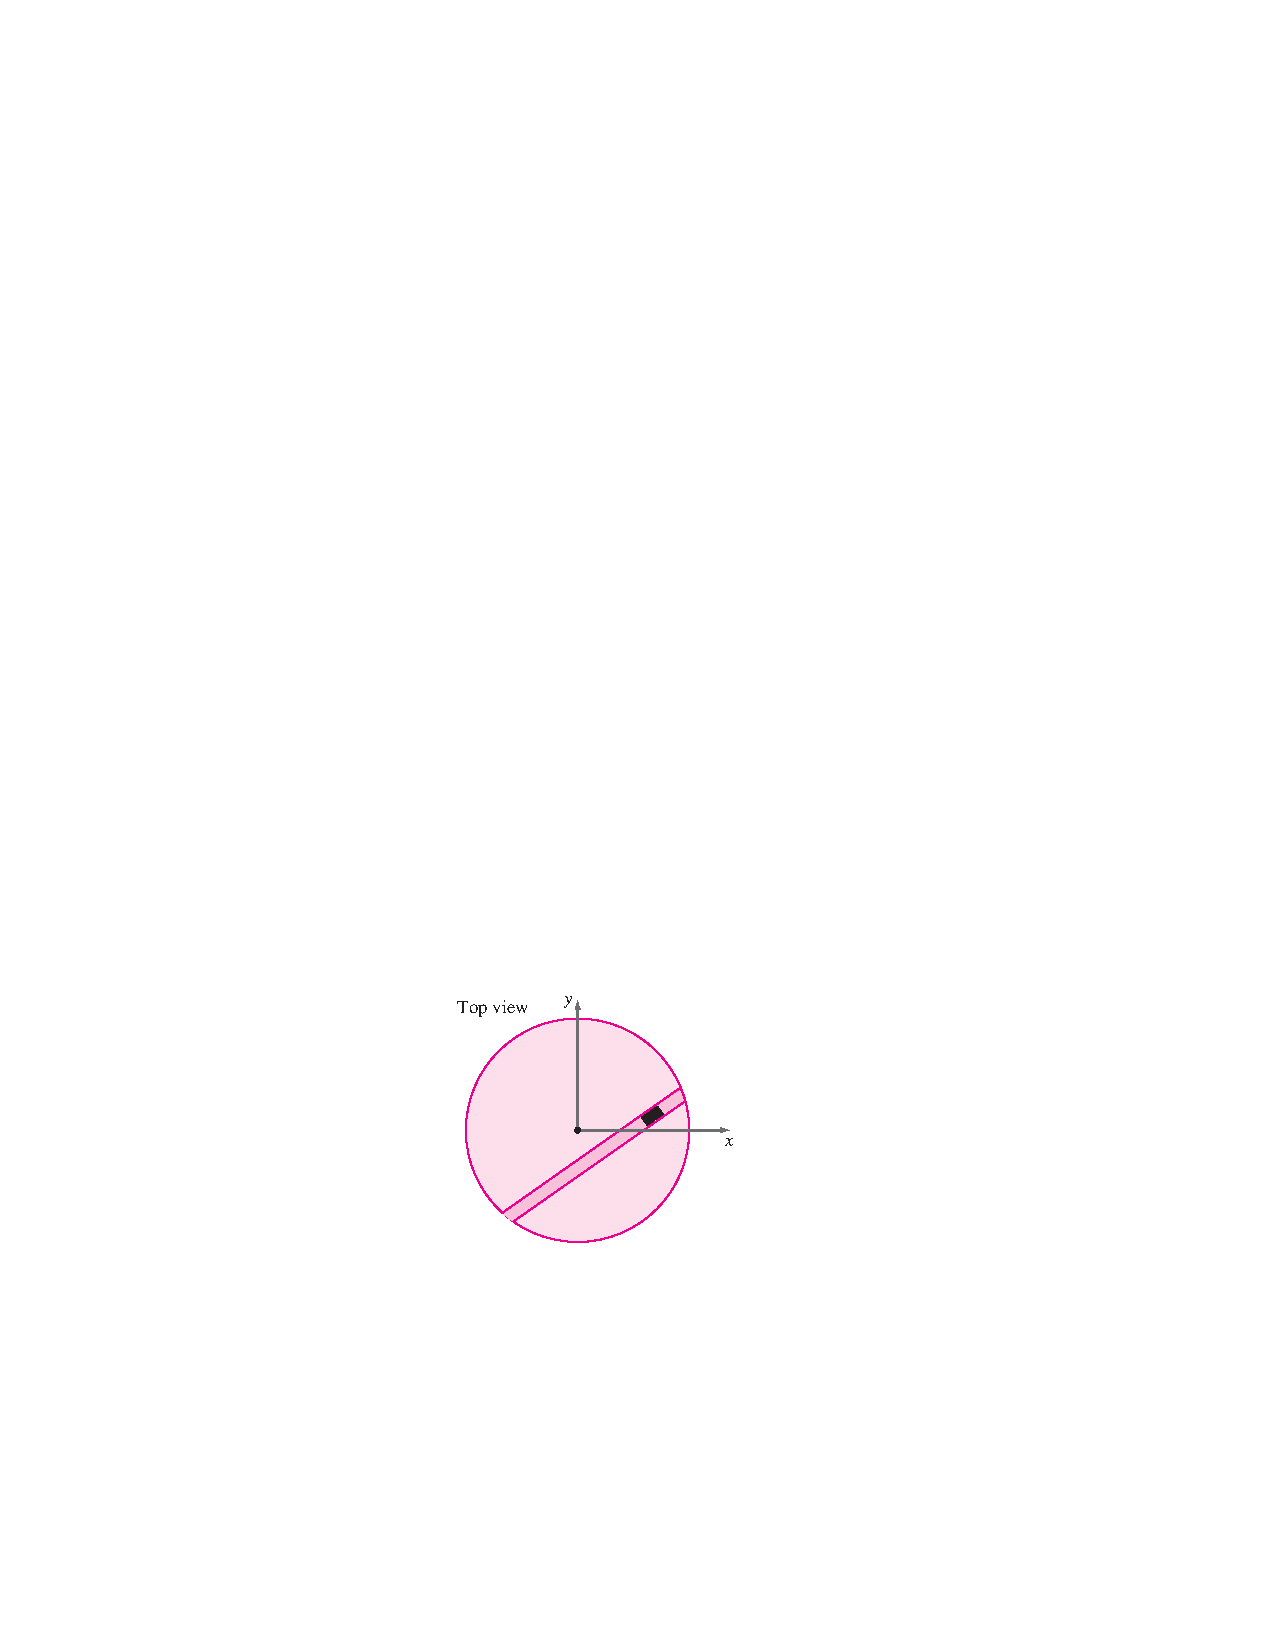
\includegraphics[width = 2.5 in]{HomeworkFigs/massinslot}}\par}



\begin{enumerate}\tight
\item  Find the acceleration of the mass in terms of $d,\theta\dot\theta,\ddot\theta, s,\dot s$ and
$\ddot s$.  Extra credit: Do this one or two more  different ways and check that all give the same answer when reduced
to $x$ and $y$ coordinates.
\begin{enumerate}\tight
\item Write the position of the mass in terms of $d,\theta$ and $s$ using base vectors
$\ui$ and $\uj$. Differentiate twice.
\item Write the position using $\uip$,  which aligns with the slot, and $\ujp$. Differentiate
twice using that $\uipdot=\vomega\times\uip=\omega\ujp$ and $\ujpdot=-\vomega\times\ujp=-\omega\uip$
\item Use the five-term acceleration formula (using $\vvsub{rel} = \dot s \uip$ and $\vasub{rel} = \ddot s \uip$).
\end{enumerate}
\item Find the equations of motion
(That is, find $\ddot\theta$ and $\ddot s$ in terms of fixed parameters and position and velocity variables.).  Do this using  AMB for the whole system about the center and
\{LMB for the mass\}$\cdot\uip$.

\item Find the equations of motion using Lagrange equations, and check for agreement.

\item Assume ICs that  $s(0)=0, \dot s(0) = v_0,  \theta(0)=0$ and $\dot\theta(0)=\omega_0>0$.
As $t\rightarrow\infty$ does $\theta\rightarrow\infty$? (As for all questions, please explain in a way that would convince a non-believer.)


\end{enumerate}

%%%%%%%%%%%%%%%%%%%%%%%%%%%%%%%%%%%%%%%%%%%%%%%%%%%%%%%%%%%%%%%%%%%%%%%%%%%%%%

\item{\bf Cart and pendulum}\label{HWcartpendulum}
A cart $m_1$ slides frictionlessly on a level surface.  A massless stick  with length $\ell$ is
hinged to it with a mass $m_2$ at the end.  Take $\theta=0$ to be the configuration when
the pendulum is straight down.  Use gravity $g$.    

\begin{enumerate}\tight

\item Find the full non-linear governing equations using Newton-Euler  (N-E, Linear and angular momentum
balance).

\item and using Lagrange. Show that you get the same equations as for N-E.

%\item Linearize the equations for small deviations from the configuration where the pendulum
%hangs straight down.
%
%\item Write the equations in standard vibration form:  $M\ddot\vx + K\vx = \vzero$.

\end{enumerate}


%%%%%%%%%%%%%%%%%%%%%%%%%%%%%%%%%%%%%%%%%%%%%%%%%%%%%%%%%%%%%%%%%%%%%%%%%%%%%%


\item{\bf Double pendulum \underline{\large \ kinematics\ }.}\label{doublependkin}
Consider a double pendulum where both links have length $\ell$. 
Consider two sets of minimal coordinates:

\begin{enumerate}
\item  Absolute angles $\theta_1,\theta_2$.  These are the angles from the vertical of the
two links.

\item Relative angles $\theta_1, \phi=\theta_2 -\theta_1$.
\end{enumerate}

Calculate the acceleration of the end of the second link in terms of the two sets, and their
derivatives.  (This is \textit{kinematics} only.  There is no place here for force, moment, free-body diagrams, mass, linear momentum,
angular momentum,  or energy.) 

\begin{itemize}
\item For the first set do this, as we have done before, by considering a non-rotating frame
that moves with the end of the first link.  This involves basic polar coordinate formulas. 


\item  For the second set, consider a reference frame that is glued to the first link. Then use
the `5-term acceleration formula' to calculate the acceleration of the end of the second link.


\end{itemize}

Show that the two methods give the same answer.


%%%%%%%%%%%%%%%%%


%%%%%%%%%%%%%%%%%%%%%%%%%%%%%%%%%%%%%%%%%%%%%%%%%%%%%%%%%%%%%%%%%%%%%%%%%%%%%%

\item{\bf Rolling cylinder}\label{HWrollingcyllinder}

A uniform cylinder with mass $m$ and radius $r$ rolls without slip outside and on top of a fixed cylinder
with radius $R$.  Gravity $g$ pulls it down. 

\begin{enumerate}\tight
\item Are the full non-linear differential equations the same as those of an inverted pendulum?
If so, or not, explain why this is expected.
\item  Assume the rolling cylinder is released from rest almost exactly at the top:   $\theta= 0^+$. At what
angle will it lose contact.  Find an analytic formula for this [Hint: use energy conservation.]  Extra: if you like, compare the result with a numerical solution of the ODEs using `events'
\end{enumerate}


%%%%%%%%%%%%%%%%%%%%%%%
\item \textbf{Rolling eccentric cylinder} \label{HWcylinder}
5730 students only.

A cylinder with radius $R$ has center of mass G offset from
the cylinder center C by a distance $d<R$. It has total mass $M$, radius $R$ and moment of inertia
$I^G$ about it's center of mass.   It rolls without slip down a ramp
with slope $\gamma$ (angle relative to horizontal), propelled by gravity $g$.


\begin{enumerate}\tight

\item Find the equations of motion.

\item Find the needed coefficient of friction to enforce the rolling constraint.

\item After release from rest, assuming it starts with the line between CoM and contact point orthogonal to the surface, how far does it roll before it skips into the air.

\end{enumerate}
It's ok to use numerical solutions based on any non-trivial parameter choices. 
No need for parameter sweeps.
\par
Interesting extension if you have \textit{lots} of time:  With appropriate initial conditions,
this can roll on a level ramp then skip, then do about a full revolution in the air,
then land with no no relative velocity at impact (thus conserving energy) and
continue rolling and skipping. This is explained, somewhat, in a paper on Ruina's
www page: ``A collisional model ...'' (figure 4 there in).  The calculation details are
like those in this paper ``Persistent Passive Hopping ...'' on Ruina's www page. I would love someone to build a model of this.   Talk with me if you are interested.

%%%%%%%%%%%%%%%%%%%%%%%
\item  \textbf{Two skates.} 
A rigid object ($m,I^G$)  moves on the plane with no gravity or other forcing.
It has on it two skates  in arbitrary position on the object and at arbitrary orientations,
with one exception. 

\begin{itemize}
\item \textbf{Special case to avoid:} The two skates have a common normal line.  This happens when in the two skates are parallel to each other, and are both orthogonal to the line connecting them.   In this one, special, excluded situation, the two skates would be redundantly applying the same kinematic constraint.  Further, in this configuration, because the two reaction forces have the same line of action, there is no dynamics or statics equation for the object which has other than the sum of the two forces; you can only find their sum, the difference between the reaction forces is indeterminate.

\item \textbf{All other cases are fine:} All other skate configurations (angles)  are ok, only the one above is problematic. 
\end{itemize}


\begin{enumerate}
\item Do this problem from beginning to end with just one skate.  Do not attempt two skates until you have mastered the case of a single skate.  If that is as far as you get, hand in your work for a single skate. 

\item Find the equations of motion using the DAE approach.  In this approach you have a 2D rigid object  with constraint forces from the skate that have associated kinematic constraint equations.

\item Find the motion by writing unconstrained Lagrange Equations (3 DoF rigid object on a plane). Then calculate generalized
forces associated with the constraints.   Then supplement the Lagrange equations with
constraint equations (two times over, once for each skate: write the skate velocity constraint and differentiate
it).  These are DAEs coming from Lagrange equations. Then solve these equations numerically using example parameters of your choosing. 



\item The solution above can also be found by simple elementary means. If you don't see this,
make an animation of the solution above.   Compare the simply reasoned result, with the numerical solution.

\end{enumerate}

\textbf{Hints:}
\begin{itemize}
\item  Again, do not try  this problem until you can do it all, from writing equations through to animation,  for a mass supported by just one skate; 
\item  Your DAEs
only enforce the constraint at the acceleration level.   Your  initial  velocities need to be consistent with the kinematic constraints. 
\item  Your
DAEs should be the same with Newton-Euler as with Lagrange.]
\end{itemize} 

\newpage
%%%%%%%%%%%%%%%%%%%%%%%

\item  \textbf{Practice  with dyadics.}  Read as much as you like, and do the exercises  in 
\bluehref{https://web.stanford.edu/class/me331b/documents/VectorBasisIndependent.pdf}{Paul Mitiguy}'s Stanford course. (Hand in a sentence about the effort you put into this.)


\item \textbf{Index notation \& Einstein Summation convention.}  For dealing with vector and tensor components and base vectors we often have one of these situations 

\begin{align*}
d=\va \cdot \vb   \qquad &d= \sum_{i=1}^3 a_i b_i  &&\mbox{dot product of two vectors}\\
[\vc] = A[\vb]   \qquad&[\vc] = \sum_{i=1}^3 A_{ij}b_j &&\mbox{matrix times column  vector}\\
C = AB \qquad        &C_{ij}= \sum_{k=1}^3A_{ik}B_{kj}  && \mbox{matrix times matrix}
\end{align*} 

where $a_i$, $b_i$ and $c_i$ are the components of vectors $\va$, $\vb$ and $\vc$; $[\va]$, $[\vb]$ and  $[\vc]$ are column vectors of their components; and $A_{ij}, B_{ij}$ and $C_{ij}$ are the components of  3$\times$3 matrices $A, B$ and $C$. 

\medskip\par
\textbf{SUMMATION CONVENTION}
\null\\
Einstein, apparently (because the rule is named after him), noticed that in these sums, the summed index always happens to occur twice in the multiplicative expression. That's $i$ in the first two examples above and $k$ in the third.  So he made up a rule to save himself the trouble of writing `$\ds \sum_{i=1}^3$'.

Here's the rule 
\bigskip
\begin{quotation}\noindent
{\bf
If a subscript appears twice in a multiplicative expression then adding up (summing), from one to three, is implied.}
\end{quotation}


So, repeating the three examples above,  using the summation convention we have that,

\begin{align*}
d= a_i b_i  \quad \mbox{means} \qquad &d= \sum_{i=1}^3 a_i b_i  &&\mbox{dot product of two vectors}\\
c_i = A_{ij}b_j \quad \mbox{means} \qquad&[\vc] = \sum_{j=1}^3 A_{ij}b_j &&\mbox{matrix times column  vector}\\
%Sum above is over j, not i,  corrected Aug 24, 2022
C_{ij}= A_{ik}B_{kj} \quad \mbox{means} \qquad &C_{ij}= \sum_{k=1}^3A_{ik}B_{kj}  && \mbox{matrix times matrix.}
\end{align*} 
 

According to these rules
\begin{itemize} 
\item You must  write "summation convention" before the first equation, for example

\bigskip
\begin{quotation}\noindent
{\bf
From this point on in this course, unless stated otherwise, we are using the summation convention.}
\end{quotation}



\item The sum is always from 1 to 3 unless you are doing a strictly 2D problem, in which case the sum is from 1 to 2;
\item If you have a repeated subscript in a multiplicative expression and you don't want to sum, you have to write 'no sum' next to the equation, for example

\[
c_i = a_ib_i \qquad \mbox{(no sum)}
\]

means that $c_1 = a_1b_1$, $c_2 = a_2b_2$, and $c_3 = a_3b_3$ which is quite different than, using the summation convention.


\[
c = a_ib_i = a_1b_1 + a_2b_2 + a_3b_3.
\]
\end{itemize}



\medskip
\textbf{FREE INDICES and DUMMY INDICES}
\null\\
There are free indices and dummy indices.  In the formula 

\[
  c_i = A_{ij}b_j
\]

$i$ is a free index and $j$ is a dummy.  Free indices survive the equation and dummies are killed off.
The equation above has no $j$ in it. Well, it looks like it's there, but it's private and not revealed in the final evaluation.   On the other hand, $i$ is free and could take on any value,
from, usually, 1 to 3.  And it survives. Thus, the equation above is really three equations,


\[
  c_1= A_{1j}b_j\centerand  
  c_2 = A_{2j}b_j\centerand
  c_3 = A_{3j}b_3 
 \]
 
\textbf{ Rules.} You can change any index to a different letter according to these rules:
 
 \begin{itemize}
 \item If it is a free index you have to change it at every occurrence on both sides of the equation;
 \item If it is a dummy index, you have to change it at both occurences in any multiplicative expression.
 \end{itemize} 
 
 For example, the equation
 \begin{align*}
 c_i &= A_{ij}b_j  + B_{ki}c_k &&\mbox{(Note: $i$ is free, and $j$ and $k$ are dummies)}\\
 \end{align*}
 
 is equivalent to all of the following equations, 
 \begin{align*}
 c_\ell &= A_{\ell j}b_j  + B_{k\ell}c_k&&\mbox{Note: change the free index $i$ to $\ell$}\\
  c_i &= A_{ij}b_j  + B_{ji}c_j &&\mbox{Note: the two multiplicative expressions do not interact}\\
   c_j &= A_{jk}b_k  + B_{kj}c_k&&\mbox{Note: a few switches.}
 \end{align*}
You should check that you agree. If you assigned any 24 numbers to each of the components on the right hand side, you should get the same values for $c_1, c_2$ and $c_3$ in all 4 of the expressions above.
 
 
 \par\medskip
 
On the other hand, if you were to write
 
 \[  
 a_i = b_j
 \]
 most likely you are talking nonsense.  If you meant it, here's what the expression says.  It says that $a_i= b_j$ for all values 
 of the free indices $i$ and $j$.  This would mean that once you knew, say, $a_1$  all  three of $b_1$, $b_2$, and $b_3$ would be equal to that.  And then, in turn, so would $a_2$ and $a_3$.   That is, the equation above would be saying that $a_1=b_1=b_2=b_3=a_2=a_3$. Unless you intend a meaning like that, which you probably do not, the free index, or indices, on both sides of any equation need to match. 
 
 \par\medskip
Rules of grammar:
 
 \begin{description}
 
 
 \item Every multiplicative expression on both sides of the equation have to have the exact same free variables. For example, if there's a free $i$ and $\ell$ on the left, then there should be a free $i$ and $\ell$ on the right.
 
 \item  Dummies can be recycled on one side of an equation and from one side to the other. For example, the following is sensible, with $i$ being a dummy, three times over, and $j$ a free variable.
 
 \[
 A_{ii}b_j  +  f_ig_ih_j  =   B_{ii}e_j .  
 \]
 
 \item An index cannot occur more than 2 times in any multiplicative expression. For example, 
 
 \[
 c_i = b_i d_je_j f_j \qquad \mbox{is nonsense}
 \]
 
 \end{description}
 
\medskip
\textbf{NONSENSE}
\null\\
If you see nonsense, stop.  Examples of nonsense:

\begin{itemize}
\item free indices are not the same on both sides of an equation;
\item free indices are not the same in different multiplicative expressions on one side of an equation; 
\item an index occurs 3 or more times in a multiplicative expression
\item unwittingly misusing the distributive law of multiplication:

\begin{description}\tight
\item   $a_ib_i = 14$ does \textit{not} imply that $b_i=14/a_i$.  (Try it with $a_1=b_1=1, 
a_2=b_2=2, a_3=b_3=3$ and note that, for example $b_1\ne 14/a_1$);
\item  $R_{ij}R_{ij}\ne R_{ij}^2$.  For starters, the left side has no free indices and the right has the 2 free indices $i,j$.  So the expression is too wrong to even check for numerical equality. A scalar is not equal to an array. 
\end{description}


\end{itemize}

\textbf{SPECIAL SYMBOLS}
To aid calculations, here are two special arrays of numbers. First and simplest is the \textbf{Kronecker delta} which is just nine numbers, all of which are 1's and 0's.

 \[
\delta_{ij} =
\begin{cases}
1 &\mbox{if}\quad i=j\\
0 &\mbox{if}\quad i\ne j
\end{cases}
\]

That is, $\delta_{ij}$ are the components of the 3$\times$3 identity matrix, with ones on the diagonal and zeros off of the diagonal.  Here are some features of the Kronecker delta:

\begin{itemize}
\item   $\delta_{ii} = 3$;
\item  $a_i\delta_{ij} = a_j$;
\item $a_ib_j\delta{ij} = a_ib_i$; 
\item   $\ue_i\cdot\ue_j = \delta_{ij}$;
\item $\delta_{ik}\delta_{kj} = \delta_{ij}$.
\end{itemize}

Check all of these and make sure they are right.
\par\medskip
Finally there is the Levi-Civita epsillon symbol, or `alternating epsillon' symbol.  This is 27 numbers all of which are 0, 1, or -1.  Actually 3 of them are 1, three are -1 and all 21 of the rest of them are 0. 

 \[
\epsilon_{ijk} =
\begin{cases}
1  &\mbox{if}\quad $ijk$ = \mbox{123, or 231, or 312 \quad (even permutations of 123) }\\
-1 &\mbox{if}\quad $ijk$ = \mbox{213, or 132, or 321\quad  (odd permutations of 123)} \\
0 &\mbox{if}\quad \mbox{$i=j$ or $j=k$ or $k=i$ \quad (not permutations of 123)}
\end{cases}
\]
The properties of $\epsilon_{ijk}$ are not so obvious as those for  $\delta_{ij}$. Here are three

\begin{itemize}
\item $\va\times\vb = a_i\ue_i \times b_i\ue_j = \epsilon_{ijk}a_ib_j\ue_k  $
\item $[\va\times \vb] =  {\cal S}([\va]) [\vb]= a^{\cal S}[\vb]$, where $[\vv]$ is a column vector of components of $\vv$ and ${\cal S}([\va])= a^{\cal S}$ is a skew-symmetric matrix with components $a^{\cal S}_{ij} = -\epsilon_{ijk}a_k$. That is, the cross product of two vectors can be calculated as the ordinary matrix product of an appropriate matrix with a vector.
\end{itemize}

\textbf{Problems.}
Assume we have defined the 3$\times$3 matrices $A$ and $B$ and column vectors $a$ and $b$ as:

\[
A=
\left[
\begin{array}{ccc}
1  & 2  &   3\\
 4 &  5 &   6\\
7  &  8 &   9
\end{array}
\right],
\quad
B = \left[
\begin{array}{ccc}
1  & 0   & 1\\
 0 &  0 &  1\\
1  &  0&   1
\end{array}
\right],
\quad
a =
\left[
\begin{array}{c}
1  \\
0 \\
2  
\end{array}
\right], \quad \& \quad
b =
\left[
\begin{array}{c}
1  \\
 1 \\
1 
\end{array}
\right].
\]



Evaluate these expressions or declare them as non sensible and explain why.


\begin{enumerate}
\item $c = a_ib_i$
\item $c = \delta_{\ell\ell}$
\item $c_i = A_{ij}b_j$
\item $c_i = b_jA_{ij}$
\item $c_i = A_{ji}b_j$
\item $c= A_{ij}B_{ij}$
\item $c= A_{ij}\delta_{ij}$
\item $ c_k = B_{jk}b_k$
\item $c_i = A_{ij}B_{jk}$
\item $C_{ik} = A_{ij}B_{jk}$
\item $\delta_{ij}\delta_{jk}\delta_{ki}\delta_{\ell\ell}$
\item $c_k = \epsilon_{ijk}a_ib_j$
\end{enumerate}






%%%%%%%%%%%%%%%%%%%%%%%
\item \textbf{Rotations.}  3D rotations are hard to visualize.  They have many representations: axis-angle, rotation vector, vector formula with cross products, dyadic representation of that vector formula, a tensor,  a matrix, Euler angles (all $n$ versions), Euler parameters and quaternians.  The notations for each of these are not universal. And for each there are the rules for composing rotations.  Add to this that the same word ``Rotation'', as for all linear transformations, can sometimes be thought of as a way to change a vector and sometimes as a way to change a given vector's representation. Most people get confused about rotations  some times.

\par
We need to describe a vector, say $\vr$,   it's components, say $r_i$ and the name of a corresponding column vector of 3 numbers, say $r$.  However, for all but the first of these we also need to know what basis we are using, say the original fixed basis $\cal F$ or a rotated basis $\cal B$.   And the same issues show for the tensor, say $\Rtensor$ or $\vec{\vec{\mathbf R}}$, its components, say $R_{ij}$ and the array of numbers used to represent it, say $R$.  Then,  we are interested in all the same things for the action of $\Rtensor$ on $\vr$, call it, say

\[  \vr^* = \Rtensor \cdot \vr  \]

[Aside:  for this write up a vector $\vr$ gets rotated to become $\vr^*$.  Another notation which we sometimes use is to start with a vector $\vr_0$ and rotate it to $\vr$. ]

Consider two frames, the fixed one  $\cal F$ with  an orthonormal basis $\ue_i$ and $\cal B$, which is $\cal F$ rotated by $\Rtensor$, with basis vectors   $\ue_i'$.     Here is a notation, including some free choices about how explicit to be about the choice of frame ($\cal F$ or $\cal B$).

\paragraph{NOTATION}
\begin{description}
\item  [$\ue_i=$]  an orthonormal set of  fixed $\cal F$ basis vectors.
\item [$\ue_i' =$] the rotated $\cal B$ basis vectors (some people call these $\hat{\mathbf b}_i$).
\item [$\Rtensor= $] the rotation, a linear transformation, that takes all vectors in $\cal F$ to $\cal B$. So

\begin{align}
\Rtensor \cdot \ue_i &= \ue_i'\\
\Rtensor \cdot \vr &= \vr^*\\
\end{align}

Three popular representations of rotation are: 

\begin{align}
\Rtensor & = \ue_i'\ue_i\\
             & = R_{ij}\ue_i\ue_j\\
              & = \un\un + \cos\theta(\onetensor -\un\un) + \sin(\theta)\ntensor          
\end{align}
where $\un$ is the axis of the net rotation and $\theta$ the amount of the rotation.
The skew symmetric tensor $\ntensor$ associated with $\un$ is such that $\ntensor \cdot \vr
= \un\times\vr$.

\item [$R_{ij} = R_{{\cal F}ij} = R^{\cal F}_{ij}=$] various notations, progressively more formal, for the components of $\Rtensor$ in the fixed $\cal F$ basis.   That is, if there is no $\cal F$ subscript or super script, it is assumed.  But if you want to be  clear that the same basis vectors are used for the left and right vectors in the dyads,  then you use superscripts and subscripts.  If you are never going to use mixed bases, then a single $\cal F$ will be good enough.
Here are various ways of thinking about the rotation matrix.

\begin{align}

R_{ij} &=\mbox{the $i$th component, in the $\cal F$ basis, of $\ue'_j$}\\
&= \ue_i \cdot \ue'_j\\
         &= \mbox{cosine of the angle between $\uei$ and $\ue_j'$}\\
         &= n_in_j + \cos(\theta)(\delta_{ij} - n_in_j)  -\sin(\theta)\epsilon_{ijk}n_k

\end{align}

\item [$R_{{\cal B}ij} = R^{\cal B}_{ij}= R^{\cal B}_{{\cal B}ij}=$] various notations, progressively more formal, for the components of $\Rtensor$ in the rotated $\cal B$ basis.  You need at least some $\cal B$ as a subscript or super script. But if you want to be super clear that the same basis vectors are used for the left and right vectors in the dyads,  then you use superscripts and subscripts.  If you are never going to use mixed bases, then a single $\cal B$ will be good enough.

\item [$R_{{\cal F}ij}\ue_i\ue_j =\Rtensor =  $] dyadic representation of $\Rtensor$ using $\cal F$ basis.
\item [$R_{{\cal B}ij}\ue_i'\ue_j' =\Rtensor =  $] dyadic representation of $\Rtensor$ using $\cal B$ basis.





\item $\vr= r_i\ue_i = r_{{\cal F}i}\ue_i = r_{{\cal B}i}\ue_i' =$ some vector of interest.
\item $\vr^*=  \Rtensor\cdot \vr 
 = r_{{\cal F}i}\ue_i' = r_{{\cal F}i}^*\ue_i = r_{{\cal B}i}^*\ue_i' =  $  the rotation by $\Rtensor$ of $\vr$.
 
 \item $R = R_{\cal F} = R^{\cal F} = R_{\cal F}^{\cal F} =[\,\Rtensor\,]_{\cal F}
= [\,\Rtensor\,]^{\cal F}=
[\,\Rtensor\,]_{\cal F}^{\cal F} =$  matrix representation of $\Rtensor$ using $\cal F$ basis.

 \item $R_{\cal B} = R^{\cal B} = R_{\cal B}^{\cal B} =[\,\Rtensor\,]_{\cal B}
= [\,\Rtensor\,]^{\cal B}=
[\,\Rtensor\,]_{\cal B}^{\cal B} =$  matrix representation of $\Rtensor$ using $\cal B$ basis.


\item $r = r_{\cal F} = r^{\cal F}   =[\,\vr\,]_{\cal F}
= [\,\vr\,]^{\cal F}=$  matrix representation of $\vr$ using $\cal F$ basis.

\item $r^* = r_{\cal F}^* =  =[\,\vr^*\,]_{\cal F}
= [\,\vr^*\,]^{\cal F}=$  matrix representation of $\vr^*$ using $\cal F$ basis.

\item $r = r_{\cal B} = r^{\cal B}   =[\,\vr\,]_{\cal B}
= [\,\vr\,]^{\cal B}=$  matrix representation of $\vr$ using $\cal B$ basis.

\item $r^* = r_{\cal B}^* =  =[\,\vr^*\,]_{\cal B}
= [\,\vr^*\,]^{\cal B}=$  matrix representation of $\vr^*$ using $\cal B$ basis.


\end{description}



\par
\medskip
\textbf{LOOK OUT FOR NONSENSE}
\null\\
If you start with a true expression, and then do legitimate operations to both sides of an equation, then you will write correct things. And with luck, a correct thing that you want.  But if you start with nonsense, or do nonsense operations, you will get nonsense.  


\begin{description}\tight
\item  $v_i$, $[\vv]$ (sometimes written as just $v$), and $\vv$ are all in reference to a given vector $\vv$.  But no two of them are equal to each other.   One is a scalar, one a $s\times1$ array, and one an abstract (or geometric) vector. 
\item Similarly,  $R_{ij}$, $[\Rtensor]$ (sometimes written as just $R$), and $\Rtensor$ are all in reference to a given tensor $\Rtensor$. But no two of them are equal to each other.   One is a scalar, one a $3\times3$ array, and one an abstract (or geometric) tensor. 
\end{description}

If one side of an equation has one of the 6 things above, and the other side a different one of the six things above, you have made an error.

\par
\medskip

\textbf{QUESTIONS.} \\
 So that you get the general idea,  the first few questions
are answered for you.   In all cases, try to derive the results from expressions that you solidly trust,
like $\Rtensor\cdot \ue_1 = \ue_1'$.

\begin{enumerate}[\bf a)]

\item  Given $\vr$ and the $\ue_i$ what is $[\vr]_{\cal F}$ = the column vector of the components of $\vr$ using the base vectors from $\cal F$?
Answer: $[\vr]_{\cal F}=\left[\begin{array}{c}\vr\cdot \ue_1 \\\vr\cdot \ue_2 \\\vr\cdot \ue_3\end{array}\right]$.


\item  Given $\Rtensor$ and the  $\ue_{i}$ find $R_{ij}$?  Answer:  $R_{ij} = \ue_{i}\cdot \Rtensor \cdot \ue_{j}$.

\item Given the $\ue_i$ and the $\ue'_i$ find $R_{ij}$?

\item  Given $R_{ij}$ and $r_i$ find $r^*_{i}$?

\item  Given $R_{ij}$ and $r_i$ find $r^*_{{\cal B}i}$?

\item  Given $R_{ij}$ and $r^*_{i}$ find $r_{i}$?

\item Given $R_{ij}$ and $r^*_i$ find $r_{{\cal B}i}$?

\item Given $R_{ij}$ find $R_{{\cal B}ij}$?

\item  Write $[\vr^*]_{\cal F}$ as many different ways as you can.

\item  Given $\underline{\underline{\mathbf A}}= R_{ij}\ue'_i\ue'_j$,  find  $A_{ij}$. Note,  $\underline{\underline{\mathbf A}}= A_{ij}\ue_i\ue_j$.

\item Pose and answer a few questions, of the general type above, that most test your remnent confusions.

\end{enumerate}

%%%%%%%%%%%%%%%%%%%%%%%
\item \textbf{Final computation project.}\label{HWfinalproject} Due at the end of the semester.
This is an extension of the double pendulum homework.  The minimal version is to simulate and animate both a triple pendulum and also a 4-bar linkage. For the triple-pendulum the equations of motion should be found three different ways. In both problems the numerical solutions should be checked as many ways as possible (Energy conservation, limiting cases where simple-pendulum motion is expected, etc). Optional extras are a) to simulate and animate more complicated mechanisms of your choice (e.g., 4,5, n link pendulum or closed kinematic loop or end link with a skate constraint) and b) to find periodic motions, c) to derive the 4-bar linkage equations by up to three methods (in total). 
\par
\medskip
\textbf{Deliverables:}

\begin{enumerate}\tight
\item Send one zip file called YourName4730.zip or Yourame5730.zip. 
\begin{enumerate}\tight
\item That should be a compressed version of a single folder.
\item In that folder should be a collection of Matlab files
\item In that folder should be a  *README file explaining how to use the Matlab files.
It should be VERY EASY to use the files for simple demonstrations
\item In that folder should be a file called REPORT.pdf.  It could be made from WORD, LateX
or scanned handwork, or any mixture of those.  It should explain what you have done, how,
and give sample output. This is the main demonstration of your effort.  As appendices this should
include your documented matlab files.
\item A video presentation of your final project. Three minutes maximum. 
\end{enumerate}
\item Your assigned exam time will start with the examiner (Ruina) watching your 3 minute presentation 
movie. 
\end{enumerate}



\item Only for fun.  Not assigned. Learn any non-algabraic ``proof'' of Euler's theorem that any ``rotation" (any motion of a sphere with the center fixed) is a rotation about an axis. Once you have learned it, write it up neatly without looking at any source.





%%%%%%%%%
\item  Consider a 90 degree rotation about the y axis followed by a $90^\circ$ rotation about the x axis.
\begin{enumerate}[\bf  a)]
\item Using geometric reasoning, find the net axis and angle of rotation as best you can.
\item Apply the axis-angle vector formula, 

\begin{equation}
\vr' =\un\  \un\cdot \vr + \cos(\theta)(\vr - \un\  \un\cdot \vr) + \sin(\theta)\un\times\vr
\end{equation}


twice in sequence, to get the new positions of unit vectors that were originally
on the $x, y$ and $z$ axis, respectively. 
\item  By taking the previous results as columns of a matrix, or by operating directly on a general vector,
find the net rotation of any vector with original components $(x,y,z)$.


\end{enumerate}



%%%%%%%
\item Write some Matlab functions 
\begin{enumerate}[\bf a)]
\item {\tt function rp = vecrot(n, theta, r)}
  % uses vector formula to calculate rotation of r given n, theta and r
\item  {function R = rotmat(n, theta)}
   % uses vector formula to calculate rotation of r given n, theta and r
\item  use {\tt  VECROT} and the matrix from {\tt ROTMAT} to calculate the rotation for some special cases.
   Check against the answers you know from geometry.
\begin{enumerate}[\bf i)]
  \item $90^\circ$ rotation about x axis,  \item $90^\circ$ rotation about z axis,  \item $120^\circ$ rotation about (1,1,1) axis. 
  \end{enumerate}
\item Write a Matlab script that takes rotation matrix as input and calculates the axis and angle of rotation. 
Check that this works forwards and back with your code from  above, both ways, with some odd examples.

\end{enumerate}

%%%%%%%%





\item Using {\tt PLOT3}, or any other way of making 3D drawings (you can use objects, drawnow,
patch, etc), 
draw a box with sides b,w, and h and a line through the box in direction n.
Then, by repeatedly using PLOT3 rotate the box smoothly rotating about axis n. Use this to illustrate 
the $120^\circ$ rotation about the axis $(1,1,1)$.

%%%%%%
%\item In lecture we found the rotation matrix for rotation about the z axis using the general axis, angle formula.
%Do the same for the x axis and find the rotation matrix associated with a rotation by all three Euler angles. 
%Check that your result agrees with any book. You may use computer algebra.

\item \textbf{Euler Angles.} Here is one set of Euler angles. The matrix representing rotation about the Fixed $x,y$ and $z$ axes are easy to construct.
Call them $R^x(\theta_x), R^y(\theta_y)$ and $R^z(\theta_z)$.  The net rotation of rotating about
the $x$ axis, then the fixed $y$ axis then the fixed $z$ axis is $R^{net} = R^zR^yR^x$.   This is also the
net rotation matrix if you rotate first about the $z$ axis, then about the new $y$ axis and then
about the newest $x$ axis.   Use  algebra, or computer algebra, to find $R^{net}$.

\item \textbf{Animation.} Draw any 3D object that pleases you in Matlab.  A box would be good.
Pick three functions of time for three Euler angles. Use anything interesting to you.  Use {\tt LINSPACE} to make three arrays of time.   Make a look that uses your solution above to make a rotation matrix at each time, apply this to your drawing and  thus animate your drawing moving in interesting ways.  Debug your program by making the angles non-zero one at a time so you can see roll, pitch and yaw independently.




%%%%%%%%%

\item  Given  the basic postulate of angular momentum balance expressed as

 \[\sum \vM_{/C} = \sum \vr_{i/C}\times \va_{i/{\cal F}} m_i\]

  show that
 
 \[
 \sum \vM_{/G} = \frac{d}{dt} \vH_{/G}  \qquad \textrm{where}\qquad  \vH_{/G} = \sum \vr_{i/G}\times \vv_{i/G} m_i.
 \]




%%%%%%%%%%%
\item \textbf {Euler equations.}  We found the equations for the general motion, at least the rotation part, of a rigid object:


\begin{align}

\Itensor &= \Rtensor \cdot \Itensor^* \cdot \Rtensor^t\\
 
 \dot\vomega  &= \Itensor^{-1}\cdot \left(  \vM_{/G} -  \vomega \times \left(\Itensor\cdot \vomega     \right) \right)  \\
\dot\Rtensor  &=  \omegatensor\cdot\Rtensor
\end{align}

where $\Itensor^*$ is the inertia in the reference state  and $\omegatensor$ is the skew-symmetric tensor version of
$\vomega$.  The $\dot\vomega$ is ambiguous, or interpretable two ways, because $^{\cal F}\dot\vomega = ^{\cal B}\dot\vomega$.   By expressing these tensors in different coordinate systems, and dotting with different base vectors, these equations can be turned into various ODEs in terms of  various representations of  $\vomega$ and $\Itensor$. 

\begin{enumerate}\tight
\item Draw a box that is long in the $x$ direction and narrow in the $z$ direction so the moment of inertia in the reference configuration could plausibly be:

\[
[I] = 
\left[\begin{array}{ccc}I_1 & 0 & 0 \\0 & I_2 & 0 \\0 &0 &  I_3\end{array}\right]
=\left[\begin{array}{ccc}1 & 0 & 0 \\0 & 2 & 0 \\0 & 0 & 3\end{array}\right].
\]

\item Simulate and animate the torque-free motion of this box using the Euler equations and the initial condition $[\vomega]_{\cal F}^0 = [0.01,\ 1.0,\  \ 0.0]'$.
Integrate for a long enough time that the motion is interesting.  Consider any other problems you like.  

\end{enumerate}

\item \textbf{Euler equations.} These are \text{the} Euler equations.  Not to be confused with the Euler eqautions above.
 Use the object-fixed coordinate system $\cal B$ based on $\ue'_i$ in which
the moment of inertia matrix is

\[
[I] = 
\left[\begin{array}{ccc}I_1 & 0 & 0 \\0 & I_2 & 0 \\0 &0 &  I_3\end{array}\right]
=\left[\begin{array}{ccc}1 & 0 & 0 \\0 & 2 & 0 \\0 & 0 & 3\end{array}\right].
\]

\begin{enumerate}[\bf a)]

\item Use the derivation of the Euler equations from lecture. These are three equations that give 
$\dot \omega_{1\cal B}, \dot\omega_{2\cal B} \ \& \  \dot\omega_{3\cal B}$ in terms of $\omega_{1\cal B}, \omega_{2\cal B} \ \& \  \omega_{3\cal B}$ and  $I_1, I_2 \ \&\  I_3$. You need not write the linearized equations.


\item Set up numerical solutions of the general non-linear free motion of such an object. That is, given initial values for the body-fixed angular
velocity components, find the body-fixed angular velocities as a function of time.

\item  As an initial condition, consider a small deviation to rotation about the $x'$ axis  

\[
[\vomega]_{\cal B} = \left[\begin{array}{c}1 \\0 \\0\end{array}\right] + 
\left[\begin{array}{c}\hat\omega'_1 \\\hat\omega'_2 \\\hat\omega'_2\end{array}\right]
\]

where the $\hat\omega'_i$ $\ll 1$ and are otherwise whatever you like.  With a plot show the time histories
of the $\hat\omega'_i$.

\item  Do likewise with rotations about the $y'$ and $z'$ axis.

\item Conclude that axis about one or more of the axes is unstable and that the others are `stable'. This is a numerical `proof by example' of the linearized ODE demonstration given in lecture.

\item Using some non-trivial initial condition, show that the solution to these equations agrees with the solutions
from the full equations with rotations.  How to compare?  Use the fixed frame $\vomega$ components and $\Rtensor$ as a function of time, from the previous problem, to find the body-fixed components of $\vomega$ as a function of time.



\end{enumerate}






%%%%%%%%%
\item \textbf{Euler Equations and then some.}  We have the great Euler equations for a rigid object:

\[
\vM_{/G} = \Itensor \cdot \vomegadot  +  \vomega \times \left(  \Itensor\cdot \vomega  \right).
\]

\begin{enumerate} [\bf a)]
\item  Write  the Euler equations entirely in terms of components and or column vectors that are entirely in the $\cal B$ basis.   For simplicity assume that  $[\Itensor]^{\cal B}$ is diagonal.

\item Set these up to solve in Matlab.   

\item Using these equations  for the evolution of $\vomega$, or the ones from the previous body-fixed representation,  set up to  solve for $\Rtensor(t)$ by setting up the evolution equations for $\Rtensor$, namely 

\[
\dot\Rtensor = \underline{\underline{\cal S}}(\vomega) \cdot \Rtensor
\]

with matrix form in the $\cal F$ frame.  Alternatively, you can assemble  the rotation matrix
as

\[

R^{\cal F} =  \left[\begin{array}{ccc} [\ue_1']_{\cal F} &[\ue]_2']_{\cal F} & [\ue_3']_{\cal F}\end{array}\right]
\textrm{\qquad and update with \qquad}  \dot \ue_i' = \vomega \times \ue_i'.
\]

\item Solve these in Matlab. Animate the motion using  some pictorial representation  you like (e.g.  a box, ellipsoid or Jack) for these problems.

  \begin{enumerate}[\bf i)]
  \item  Pick some object and initial conditions that interest you.
   
  \item  Consider an initial condition near to rotation nearly about the intermediate axis.
  
  \item Wobbling of a plate (See problem \ref{Feynmanplate}).
  
  \end{enumerate}
  
  In each case you may want to make other plots, or show the trajectories of some special
  points, in order to clarify some statement you want to make (like about the relative rotation
  rates of the plate normal and of the whole plate).
  
  \item Instead of representing the rotation with a rotation matrix use Euler angles.  That is write the equations of 
  motion using Euler angles and show at least one example where your solution agrees with the rotation matrix solution.

\end{enumerate}

%%%%%%%%%%
\item \textbf{Static and Dynamic Balance.} A rigid object is mounted rigidly to a fixed axis that has bearings \textit{on} the $x$ axis.  That is, 
\[\vomega = \omega \ui =  \mbox{constant.} \ne \vzero\]
\textit{``Balance''} in this context means that the net force $\vF^{tot}$ and moment $\vMsub{C}^{tot}$ are zero

\[ \vF^{tot} = \vzero \qquad \centerand \qquad \vMsub{C}^{net} = \vzero. \]

These are the total force on the object from the bearings and from any other forces or moments applied. That is, in a state of `balance', the bearing reactions exactly cancel any other applied forces and moments, and nothing more.   In these equations, the moment can be measured relative to any convenient fixed  point C, typically one uses  a point on the axis.  

\begin{enumerate}[\bf a)] \tight
\item  \textit{Static} balance means $\vF^{net} = \vzero$.  Name precise conditions on the type of object, or location or orientation of the object that make it so static balance is achieved. Hint: (separate from looking at lecture notes) Use Linear Momentum Balance.
\item Describe a simple experiment to detect static balance.  You can assume that you can disconnect the motor that causes $\vomega$ and that the bearings are very low friction.
\item  \textit{Dynamic} balance means that both $\vF^{net} = \vzero$ and $\vMsub{C}^{net} = \vzero$ . Describe precise conditions, in terms of the type of object, position of the object, or orientation of the object, so that dynamic balance is achieved.
\item Consider the most unsymetric object you can.  For how many different positions and orientations can this object spin with dynamic balance?  Describe them.
\item  Consider this object.  A rigid massless plus sign has four unit masses at the points $\pm 1$ on the $x$ and $y$ axis.  It is rotated  30\degrees counter-clockwise about the $z$ axis.  This object is spun about the $x$ axis with $\vomega = \omega \ui =  \mbox{constant.} \ne \vzero$.  Show that this is dynamically balanced two ways:  I. Using the moment of inertia, and II. adding up the moments and  forces due to each of the 4 masses.  Hint: for point C use the origin, the middle of the rotated plus sign. 
\item Consider an unknown object spinning on a shaft at constant rate.  The object is entirely between
the bearings (totally between two parallel planes, both planes orthogonal to the axis and each plane passing through a bearing).  It is claimed that there is
only a reaction force at one end of the shaft, and none at the other.  Is this possible?  If not, prove it.
If so, find an object where this is possible (pick dimensions for the bearing locations and the the
object mass distribution). \par
\hfil 
\includegraphics[width = 4.55 in]{Homeworkfigs/DynamicBalance.pdf} 
\end{enumerate}
%%%%%%%


%%%%%
\item \textbf{Spinning Satellite.}  \label{satellite1}\\

\begin{enumerate}\tight
\item []  Compare three satellites: 
\begin{itemize}\tight
\item [*] All three Satelllites consists of  uniform-density ($\rho$ = 1) objects welded together: a unit cube and  spheres each with radius 0.5.   
\item [*]The spheres are welded to the middles of cube faces, just touching at one point. \\ 
\item [*] In the defining configuration, the cube corners are at $x,y,z = 0$ or $1$. \\ 
\item [*] All satellites have a massless antennas, which go from  (0,0,0) to (3,3,3) and an the other from
(0,0,0.5) to (2,2,0.5).
\end{itemize}

\item  Satellite  A has two spheres welded to the surfaces with outward normals in the $+x$ and $+y$ directions;
\item Satellite  B  has a the third sphere on the $+z$ face; and
\item Satellite C has spheres on all 6 faces.



\end{enumerate}
\noindent
Things to do: 
\begin{enumerate}[\bf i)]
\item Find the centers of mass of the sattelites.
\item  Find the moments of inertia matrix relative to the center of mass.
\item  Find the three principle moments of inertia (2 are the same for satellite A, why?)
\item Animate these  satellites tumbling in space (take care that the centers of mass are stationary).
\begin{enumerate}[I:]
\item rotating about each principle axis
\item The most arbitrary motion you can find.  Look at the motion of the antenna tips.
Can you describe this motion in a simple way?
\item If the answer to the problem above is in any way simple, can you find it by pencil and paper reasoning?
\end{enumerate}
\end{enumerate}

%%%%%%%%%%%%%%%%%
\item
\label{Feynmanplate}
See \bluehref{http://www.youtube.com/watch?v=dQai9QikTBI}{this video} from minute 10:05 to 11:03.
 Does Feynman have it right? That is your HW problem.  At a minimum, use your 3D simulator to see if you get the motion he describes.  To check this you have to compare the rate of wobbling of a normal to the plate to the rate of rotation of a drawing on the plate.   If you want to do something analytical,   assume a steady precessing solution of a flat plate.
Keep clear in your head the relation between these three angular velocities: precession, spin and total.  




\item \textbf{Spinning Satellite: Part II.}   \label{satelite2} This problem picks up on the observations in problem \ref{satellite1} and asks for a bit more rigor. You might have already answered some of these questions when doing problem \ref{satellite1}, and might not have got to them. Here is a chance to learn it all.


Here are some claims about satellites, A,B and C from problem \ref{satellite1}:

\begin{enumerate}[A)]

\item Satellite A.
\begin{enumerate}[i.]
 \item Has three unequal principle moments of inertia, rated from biggest to smallest as 1, 2, and 3.  
 \item The intermediate moment of inertia is parallel to the line connecting the centers of the two spheres.
 \item All of these are possible motions of the free satellite:

 \begin{itemize}
 \item exactly rotating  about axis 1 or 2 or 3.
 \item  wobbling about axis 1 or 3.
 \item  wobbling about axis 2, but flipping occasionally.  In this motion  a directed line segment  in the object, in the +2 direction, will wobble, the point approximately in the -2 direction, then wobble and then reverse.
 \item  The motions above are all of the possible motions.
 \end{itemize} 
 
\end{enumerate}

\item  Satellite B.
\begin{enumerate}[i.]
 \item Has two equal principle moments of inertia, so is dynamically axisymmetric.
 \item The  symmetry axis is in the (1,1,1) direction. 
 \item All of these are possible motions of the free satellite:
 \begin{itemize}
 \item exactly rotating  about the symmetry axis or about any axis perpendicular to the symmetry axis;
  \item  steady precession about the symmetry axis,

 \item  The motions above are all of the possible motions.  For example, there is no wobbling about any other axis.
 \end{itemize} 
\end{enumerate}

\item  Satellite C.
\begin{enumerate}[i.]
\item Is dynamically a sphere;  every direction is a principle direction.
\item No matter what the initial condition, the motion is always with constant $\vomega$. There are no precessing motions.
\end{enumerate}

\end{enumerate}

 Rate all of the statements above as true or false. Justify your answer using computer calculations or simulations, or using reasoning based on the equations of mechanics. Be as convincing as you can be, within the time you want to allot to the problem. One useful thing is to track the trajectory of the tip of an appropriate line segment that is fixed in the satellite (say, the tip of one of the specified antennae, or some other antenna that you add). You don't need to hand in a simulation for each and every case. You can simply state what you observed in the simulation using clear-enough words that your answer seems convincing.
 


%%%%%%%%%%
\item \textbf {Steady precession is general for an axisymmetric object in space?}  This reinforces one point made in problem \ref{satelite2}.
If you covered it well enough already, you can skip this. For an axisymmetric object floating in space we found steady precessional motions.  Are these the most general motions of an axisymmetric object in space? Yes or no. Make a convincing argument, numerical, analytical, or abstract, for your answer.



%%%%%%%%%%
\item \textbf{Steady precession of a top.}   Assume an axisymmetric top with mass $m$ and principle inertias $I^G_1=I^G_2$ with $I^G_3$ arbitrary but non-zero.
The center of mass G is a distance $d$ from the stationary pivot at O.    This problem concerns steady precession solutions with   $\ueiii'$ making a constant angle $\theta$ with the
upwards $\uk$ direction.  The top symmetry axis $\ueiii'$ precesses with constant rate $\omega_p$ around the $\uk$ axis.  Relative to the precessing reference
frame, the top spins with  $\omega_s$ about the $\ueiii'$ axis.   That is, at all times the angular velocity of the $\cal T$op is

\[
\vomega_{\cal T/F} = \omega_p \uk  + \omega_s\ueiii'
\]

\begin{enumerate}\tight
\item  Find steady precession motions of this top.  That is, given $g,d,m,I^G_1$ and $I^G_3$ what restriction(s) do the laws of mechanics put on $\theta,\omega_p$ and $\omega_s$.

\item   Assume such precession is very close
to upright ($\theta\ll1$).  What is the slowest spin, for given mass and inertia parameters, for which such steady precession solutions exist.  This is a non-rigorous guess for the  critical spin speed for upright stability.

\item Are these the most general motions for an axisymmetric top with gravity?  You can get a definitive answer to this question using your existent simulator, just adding in a torque from gravity. 
\end{enumerate}




%%%%%%%
\item \textbf{Steady precession of a Disk on plane with gravity.} We assume here steady motions with constant lean angle $\theta$ and constant pitch rate $\omega_s$. In the steady motion the center of mass of the disk traverses a circle with radius $R$.  Given disk radius $r$,
mass $m$, gravity $g$ and inertia  matrix in the disk frame, with $\ueiii'$ orthogonal to the disk plane,

\[  \left[\begin{array}{ccc}I_1=I & 0 & 0 \\0 & I_2=I & 0 \\0 & 0 & I_3=2I\end{array}\right] .\] 

The laws of mechanics, with the contact conditions, give  restrictions
on the radius of the circular motions $R$, $\omega_s$, the precession rate $\omega_p$, and the lean angle $\phi$.  Find these for these cases:
\begin{enumerate}\tight
\item  All solutions with no slip
\item All solutions with no friction.
\item The intersection of the two (all solutions with no slip and no friction), these are the most famous ones.
\end{enumerate}

\item \textbf{Spinning top  in 3D.} Find, solve and animate solutions for a spinning top  in 3D.  Use Euler angles.
Check that, when used as initial conditions, the steady precession solutions (above) yield steady precession. 
 Is the critical speed for the steady precessing solution indeed the minimum stable upright speed for the full 3D solutions? Investigate this either
 numerically, analytically, or both.

\end{enumerate}
\end{document}



%%%%%%%
\item \textbf{Rocket.} 2D simulation of a rocket.
 \hskip -2 in \vtop{
\begin{itemize}\tight
\item[$ d = $] distance from fins to CoM

\item[$\theta =  $] angle of fins relative to parallel to rocket $= \theta(t)$

\item[$ T  = $] thrust, parallel to rocketv$ = T(t)$

\item[$g =  $] gravity constant

\item[$ m, I = $] mass and moment of inertia about center of mass

\item[$A  =  $] area of fin,  $\rho =$ fluid density

\item[$ c1, c2 = $] coefficients you use in your circular lift-drag polar for the fins.
\end{itemize}
}\\

 
\begin{enumerate}[\bf a)] 
\item  Pick numbers and functions that you like and make an animation that satisfies the equations of motion

\item If you have time, make $T$ and $\theta$ controllable with your keyboard. Then, find parameters and a task that you can achieve by playing your video game.    
\end{enumerate}
 

\textbf{NOTES:} 

\begin{itemize}
\item This model will not hover well.  That is, I don't think you can stabilize hovering with this model because the fins have no effect in hovering.  If you were to try to stabilize hovering it would be a complex thing, like unicycle balancing, involving cyclical motions.

\item A trick to try for would be launching from ground and doing a loop without crashing. You'll have to fly pretty high before turning around for the loop, otherwise you'll crash. Then flying straight up afterwards.

\item  For interactive ODE solution you shouldn't try to use ODE45.  Easiest to use your own Euler integrator that queries the keyboard at every time step.
\end{itemize}
\newpage

%%%%%%%
\item \textbf{Airplane} 2D interactive simulation. 
This adds a second wing to the rocket.
Look at, and use in your work, the variables, variable names, and lift and drag model, on the next page.   Values are  in consistent units, \eg meters, kg,  and s and units derived from these,
like N, m$^2$, etc.\par


\hfil 
\includegraphics[width = 4.55 in]{Homeworkfigs/planeparameters.pdf}
 



\begin{enumerate}[\bf a)]
\item Plot lift and drag (normalized by $\rho A v^2$) vs angle of attack $\alpha$ for $0\le\alpha\le2\pi$
\item Make a `cross plot' of lift vs drag.  This is also called a `lift, drag polar'.
\item Generally lift is considered good, and drag is considered bad. We want more good than bad, so quantify the goodness of a wing by its  \textit{lift-to-drag ratio}, $L/D$.  Good wings, sails, keels and tires have high lift-to-drag ratios.  Like, 100 for a super glider.  The  keel of an old boat might only  have L/D of something like 1/3.  Lift-to-drag ratio is a function of $\alpha$. Plot it for the wing in this model.
What is its maximum value and at what value of $\alpha$.  
\item Set up, on paper, the calculation of the various time-varying quantities in terms of state variables, constants and controls.
\item Made a 2D numerical simulation and animation of a glider ($\theta_T =$ constant, and $F_p = 0$). 
\item Find at least one steady gliding solution.
\item 5710 only: Find the best gliding solution you can.  This is the one for which the glide angle (deviation from horizontal of $\vv_G$) is minimum.  What is $\theta_T$ for this best glide?  What is the best glide angle?
\item  5710 only: How does the tangent of the  best glide angle compare to the best lift to drag ratio (above)?
 How would you have to change the plane design to get the best glide angle to match the best lift to drag ratio?
\item Make a 2D simulation of the powered and controlled plane.  Use the left and right arrows to adjust the propeller thrust.
Use the up and down arrows to control the elevator (Tail) pitch.
\item What is the highest steady climb rate you can achieve (highest steady $\dot y$)?
\item Learn to fly your plane.  Can you land it?  Fly it upside down? Do a loop?


\end{enumerate} 


\newpage

\par

{\footnotesize
\underline{\textbf{Constants:}}
\begin{enumerate}\tight \setlength{\itemindent}{.75in}
\item[$  m=500$] = mass of plane
\item[$ I= I^G = 1000$] = moment of inertia of plane about center of mass
\item[$ g  =10 $] = gravity acceleration
\item[$ \rho =1$] = density of air
\item[$  d_w=0.25$] = distance from G back W, the  center of Wing lift
\item[$  d_T=4$] = distance from G back to T, the center of tail/elevator lift
\item[$  A_W=20$] = area of wing
\item[$  A_T =4$]  = area of horizontal stabilizer (tail)
\item[$ F_{max} =5000$] = maximum thrust of propeller
\item[$  C'_L, C'_D$] = coefficient for finding lift and drag  coefficients: $C'_L = 1, C'_D= 0.02$ 
\item[$\theta_{Tmin}, \theta_{Tmax} $] =minimum and maximum horizontal stabilizer angle relative to plane = $\pm 15\degrees$

\end{enumerate}

\underline{\textbf{State Variables:}}
\begin{enumerate}\tight\setlength{\itemindent}{.75in}
\item[$  x_G, y_G = $] Position of center of mass, $\vrsub{G}=x_G\ui + y_G \uj$
\item[$  \theta_p=$] Angle of plane, $\ul= \cos\theta\ui + \sin\theta\uj$
\item[$  v_{Gx}, v_{Gy}=$] Velocity of center of mass, $\vrsub{G} = v_{Gx}\ui+ v_{Gy}\uj$
\item[$  \omega=$] angular velocity of plane, $\vomega = \omega \uk$
 \end{enumerate}

\underline{\textbf{Controls:}}
\begin{enumerate}\tight
\item[$\theta_T =$] angle of horizontal elevator relative to plane: $  \theta_{Tmin}\le \theta_T\le \theta_{Tmax}$.  \\ Note $\theta_T$ is commonly slightly negative in steady level flight (to make negative lift, to  balance sum of moments about W). 
\item[$ F_p=$] thrust of propeller.  $0\le F_p\le F_{max}$, along the plane:  $\vF_p = F_p\ul$.
 \end{enumerate}

\underline{\textbf{Other time-varying variables:}}

\begin{enumerate}\tight
\item[\bf Note:] all of these need to be calculated at every time step
\item[$ \vv_W =$] velocity of wing (at center of lift)
\item[$  \vv_T =$] velocity of Tail (at it's center of lift)

\item[$  \alpha_W = $] angle of attack of wing 
\item[$  \alpha_T = $] angle of attack of tail 

\item[$  L_W, D_W=$] lift and drag on wing, $\perp$ to, and anti-parallele to $\vv_W$: 

\begin{align}
L_W &= \frac{1}{2}\rho A_W |\vv_W|^2 \overbrace{ C'_L\sin(2\alpha_W)}^{C_L}\\
D_W &= \frac{1}{2}\rho A_W |\vv_W|^2 \underbrace{( C'_D + C'_L(1-\cos(2\alpha_W))}_{C_D}
\end{align}



\item[$  L_T,D_T=$] lift and drag of tail tail, as for wing, but using $\alpha_T, \vv_T, A_T$

\item[$  a_{Gx}, a_{Gy}=$] Velocity of center of mass, $\vasub{G} = a_{Gx}\ui+ a_{Gy}\uj$
\item[$  \dot\omega=$] angular acceleration of plane, $\dot\vomega = \dot\omega \uk$ 
\item[$\vF_W =$]  the net force of air on the wing.  This comes from lift and drag, perpendicular and parallel to $\vv_W$ 
\item[$\vF_T =$]  the net force of air on the wing.  This comes from lift and drag, perpendicular and parallel to $\vv_T$ 

\end{enumerate}
}

\textbf{Note:}  There are 6 different relevant directions, no two of which are generally parallel nor perpendicular:
$\ui, \ul, \vv_G, \vv_W, \vv_T $ and the tangent to the tail ($\theta_T$ counterclockwise from $\ul$).
And, 3 more directions perpendicular to some of these, namely: $\ui$ (the $y$ coordinate), 
$\vv_W $ (the direction of wing lift) and $\vv_T$ (the direction of tail lift). 9 in all.



%%%%%%%%%
\item \textbf{Stability of bouyancy.}  Consider a  box shaped boat: a  rectangular prism.  That's a box $w\times \ell$ and $h$ tall.  It has uniform density $\rho_b$.  It is in equilibrium (not necessarily stable) floating vertically ($h$ is up and down) on  water with density $\rho_w>\rho_b$. 
\begin{enumerate}
\item `` What is the \textit{draft} (or \textit{draught}) of  your  box boat, or  ``How much does it `draw'?"  That is, how much is under water?  Or, what is $h_w$, the depth of box under water?  In boat lingo this is  Your answer is:\\
``The box draws (or, `draft is') $h_w=$ (some expression using $\rho_w,\rho_b,\ell,w$ and $h$).''
\item How big a moment $M$, applied along the length (a moment to tip the boat)  is needed to hold the boat tipped an angle $\theta$? about the longitudinal (lengthwise, $\ell$) direction.   Note, $M>0$ for a stable boat and negative for an unstable boat.
\begin{enumerate}
\item Calculate assuming $\theta\ll 1$ using Euler's method (based on motion of body-fixed centroid with an additional moment from the moment of inertia at the waterline).
\item Challenge: Calculate by finding the tipped centroid (probably a numerical calculation) and plot vs $\theta$, comparing this exact solution with the Euler approximation. 
\item Give the conditions on $\rho_w,\rho_b,\ell,w$ and $h$ for having a stable vertical boat?  Draw a picture, scaled correctly,
of a boat sized so that it is on the margin of stability ($M=0$) assuming $\rho_w = 5\times$ row boat :). 
\item Challenge:  Considering both vertical force and tipping moments animate a bobbing box. Various challenge levels:
\begin{enumerate}
\item  2D vs 3D
\item Full calculation of submerged volume and centroid location vs  Euler small rotation (and small vertical displacement) theory.
\item For added realism,  still without doing full fluid mechanics calculations, people often partially account for fluid flow by  using
`added mass'.  This is not added weight, it is added mass in the dynamics.  For \bluehref{http://www.vibrationdata.com/tutorials2/added_mass_fluid.pdf}{this problem} the appropriate added mass would be
on the order of $m_{added}\approx 0.7 \times m_b =0.7\times \rho_b \ell w h$.  One can also add a fluid damping term.\end{enumerate} 
\end{enumerate}
\end{enumerate}

\item \textbf{Sailing, 2D, looking down.}  Assume both the sail and keel of a sailboat have the properties of the wing in the airplane problem.
But,  the  density of the water is 1000 times the density of the air.   The wind is coming from the north at speed $v_{windtrue}$.
You get to pick the angle of the boat, the angle of the sail, and the areas of the keel and sail.  What is the absolute fastest you can make the boat have
steady sailing  (something $\times v_{windtrue}$? For this sailing, what are all the areas of keel and sail and what are the orientations of the boat and sail and path. You can try to do this analytically.  Or, you can use Matlab optimization and see the best you can do.  Or, you can use successive guessing.  Start with guessing until you understand the question better.

%%%%%%%%%
\newpage
\item \textbf{Robot Arm:  forward kinematics.} Make up a robot arm with up to $N = 6$ links in 3D. Pick whatever numbers you like and whatever shapes you like for animation.  Animate it's motion as the joint angles are varied interesting ways.  Also, calculate all of the link angular velocities, angular accelerations and the positions and accelerations of the centers of masses.  

\par\noindent
\textbf{Basic Notation}
\begin{itemize}
\item Links are numbered $i$, from 1 to $N$, the next two  links are $j=i+1$ and $k = j+1$ (think, .e.g.,  $i=7, j=8,k=9$);
\item The parent hinge of link $j$, connecting it with link $i$, the one it rotates around,  is labeled hinge $j$; 
\item The child hinge of link $j$, connecting it with link $k$, the one $k$ rotates around, is labeled hinge $k$;
\item The Center of Mass of link $i$ is at $G_i$;
\item Each link $i$ has associated object-fixed frame with origin at point $i$ whose
rotation relative to the fixed frame is $\Rtensor_{\, i/\mathcal{F}}$, or $\Rtensor_{\,i}$, for short;
\item The orientation  of hinge $i$ is $\un_i$, and the rotation angle of that hinge, of link $i$ relative to $i-1$,  is $\theta_i$;
\item Other quantities of interest are relative positions $\vrsub{G_i/i}, \vrsub{(i+1)/i}$, relative velocities $\vvsub{G_i/i}, \vvsub{(i+1)/i}$,
and relative accelerations $\vasub{G_i/i}, \vasub{(i+1)/i}$.
\item Also, of interest are the absolute angular velocities and accelerations of the links, $\vomega_i$ and $\valpha_i$. For dynamics we also need $m_i$ and $Itensor_i$ (about CoM).

\item The reference configuration:
\begin{itemize}
\item Superscript $^0$ indicates the reference configuration:  
\item $\theta_i^0=0 $;  (joint angles are all zero in reference configuration)\\
 $\Rtensor_{\, i}^0 = \onetensor$ (all links have no rotation relative to the fixed frame, in the reference configuration); Also, $\Rtensor_{\,0}=  \Rtensor_{\, \mathcal{F}/\mathcal{F}}=\onetensor$ (the base doesn't rotate, for all time);
\item Other values in the reference configuration: $(thing)^0$
\end{itemize}

\end{itemize}

\hbox{\hsize = 6 in
\hskip 0 in
\vbox{\hsize = 1.5 in 
\textbf{Left:} Robot arm.\\
\textbf{Right:} One link of a robot arm with at least 8 links.
\vskip 2 in }
\vtop{\hsize = 1.5 in 

\includegraphics[width = 1.5in]{Homeworkfigs/robotarm}}
\hskip .5 in
\vtop{\hsize = 2 in 
\includegraphics[width = 2.5in]{Homeworkfigs/robotlink}}\hfill
}

\newpage

\textbf{Forward kinematics problem:}\\
\textbf{Given:} everything about link $i$, that's $(everything)_i$, and\\
\phantom{\textbf{Given:}}  everything in the initial state, that's  $(everything)^0$, and\\
\phantom{\textbf{Given:}}  everything about the next hinge's, $j=i+1$, rotation, that's $\theta_{j}, \dot\theta_{j}$, and $\ddot\theta_{j}$, \\
then \textbf{Find:} \ \  everything about link $j$, that's $(everything)_j$.


\par\noindent
\textbf{Matlab hint:}\\
One way to keep track of things is to  make lots of matrices, one for each variable or vector. Each column corresponds to a link.
That is,  {\tt rGrelParent(:,5)}  would be the components of $\vrsub{G5/5}$).  For the rotation matrices you can either use 3-index arrays, or string out the matrices into 9-element column vectors.  So that you can use the same algorithm on the
first and last link, you can create some physically useless things: 1)  A completely stationary link 0, for which you fill in simple values that remain constant at all time;
2) A useless last link, after the `hand', so that you can place a hinge on it (give it no mass and, when the time comes, don't calculate torques for it).


\paragraph{Suggested order of work}
\begin{enumerate}[\bf a)] \tight
\item  Ignore all terms involving time. That is, skip everything to do with $\vv, \va,\vomega$ and $\valpha$ and $\Itensor$
\item Just do one object.  But try it with a crooked $\un^0_1$ (that is, not aligned with $\ui,\uj$ or $\uk$).  Animate it.
\item Then, one more object.
\item  Then $n>2$ objects.  Note, if $n>2$, you can give the first link no mass, no inertia and no length.  The first two hinges simulate a U-like-joint.  If $n>3$, you can give the first two links no mass, no inertia and no length.  The first three hinges simulate a ball-joint. In both cases, make the hinge axis mutually orthogonal. 
\item Then add calculation of other things ($\vv, \va,\vomega$ and $\valpha$ and $\Itensor$) and see if you can check that they are reasonable.
\end{enumerate}
\par




\paragraph{Kinematics Algorithm.}
We work our way out from base to tip. We imagine applying the hinge rotations, one at  a time. Each time the rotation applies  to the whole remaining set of links in the arm.  Imagine starting with a 3-link straight arm, first bend the shoulder and do all calculations, then the elbow, then the wrist.
Below, assume we have already figured things out to link $i$, and now want to find things for the next link $j=i+1$. Each of these steps you have seen before, or should be able to derive from the `Q-dot` formula ('the transport theorem').

\newpage
\paragraph{Steps, in order:}
{\large
\begin{align}
\vrsub{j} &= \vrsub{i} + \vrsub{j/i};\\
\vvsub{j} &= \vvsub{i} + \vvsub{j/i};\\
\vasub{j} &= \vasub{i} + \vasub{j/i};\\
\un_j &= \Rtensor_i \cdot \un_{j}^0, \textrm{the new hinge rotates with the previous link};\\ 
\Rtensor_{\,j/i} &= \Rtensor(\un_{j},\theta_j), \textrm{that's the axis-angle formula for the rotation matrix};\\
\Rtensor_{\, j} &= \Rtensor_{\, j/i} \cdot \Rtensor_{\, i},  \textrm{the new link gets  rotated further by the new hinge};\\
\vr_{G_j/j} &=  \Rtensor_{\, j}\cdot \vr_{G_j/j}^0;\\ 
\vr_{k/j} &=  \Rtensor_{\, j}\cdot \vr_{k/j}^0;\\ 
\vrsub{G_j} &= \vrsub{j} + \vr_{G_j/j};\\
\vrsub{k} &= \vrsub{j} + \vr_{k/j};\\
\vomega_{j/i} &= \thetadot_j \un_j;\\
\vomega_j  &= \vomega_i + \vomega_{j/i};\\
\valpha_{j/i} &= \thetaddot_j \un_j; \textrm{here, the subscripts label objects}\\
\valpha_j &= \valpha_i + \valpha_{j/i} + \vomega_i \times \vomega_{j/i}, \textrm{ from  the Q-dot formula applied to $\vomega$'s.};\\
\vv_{G_j/j} &= \vomega_j\times\vrsub{G_j/j};\\
\vv_{k/j} &= \vomega_j\times\vrsub{k/j};\\
\vvsub{G_j} &= \vvsub{j} + \vv_{G_j/j};\\
\vvsub{k} &= \vvsub{j} + \vv_{k/j};\\

\va_{G_j/j} &= \vomega_j\times\vvsub{G_j/j} + \valpha_j\times \vrsub{G_j/j};\\
\va_{k/j} &= \vomega_j\times\vvsub{k/j} + \valpha_j\times \vrsub{k/j}, \textrm{or you can use the $\vomega\times\vomega\times \dots$ version};\\
\vasub{G_j} &= \vasub{j} + \va_{G_j/j};\\
\vasub{k} &= \vasub{j} + \va_{k/j};\\

\Itensor_j &= \Rtensor_{\, j}^T \cdot \Itensor_j^0\cdot \Rtensor_{\, j}, \textrm{needed for dynamics, not for kinematics}.

\end{align}
}

\par\noindent
These 20-some  things have lots of redundant information. Some steps could be combined.  But, they are all laid out here, in small steps, so you can see the logic of each step.   Also, by calculating all these things, and saving them,    you have less to calculate and think about when you do the animation and the mechanics.  

\par 
 I guess that the
computer time required might be reduced by something like a factor of 10 if all redundancies were removed and fancy compact notation was used (like Featherstone's `spatial vectors', or Denavit-Hartenberg (DH) parameters and `homogeneous' transformations), but these have additional overhead in terms of setup and understanding.


%%%%%%%%%%%%%%%%%%%
\item \textbf{Robot arm``Inverse'' Dynamics problem:}\\
For a given motion, knowing all joint angles, rates and accelerations, and having the solution to the kinematics at your fingertips,  you can find all of the joint torques by the following.

\begin{enumerate}\tight
\item Draw a FBD of the last link, 6.
\item Write AMB with respect to a point on hinge 6. Dot this equation with $\un_6$.  This gives the joint 6 moment $M_6$.
\item Draw a FBD of joints 5 and 6. Calculate AMB with respect to point 5.  Dot with $\un_5$ to get $M_5$.
\item Then joints 4,5, and 6.  Etc

\end{enumerate}


 \item \textbf{Robot arm ``Forwards'' Dynamics.}\\
 Assume we have column vectors for the angles, rates, accelerations and torques: $\hat\theta, \dot{\hat\theta}, \ddot{\hat\theta},\hat M$
 The general form of the equations of motion turns out to be this, you can convince yourself of this by looking at the forwards dynamics.    
 
 \[
 A(\hat\theta) \cdot \ddot{\hat\theta} =  \hat F(\theta,\hat\theta, \dot{\hat\theta})  + \hat M
 \]
 
 $A$ is the \textit{mass} matrix.  $\hat M$ are the joint torgues, and $\hat F$ is everything else, including gravity and any forces applied to the robot.  The key is that these equations are linear in $\hat\theta$.
 
 We could try to build up this equations symbollically by setting up the``inverse'' dynamics problem. Then we could pull out the 
 mass matrix by looking at the coefficients of the $\ddot\theta_i$ in the equations.
 
Instead, we can pull out the mass matrix  numerically by doing a sequence of imagined ``inverse'' dynamics problems.

Recipe:

\begin{enumerate}\tight
\item  Do the "inverse'' dynamics problem, setting all of the $\ddot\theta_i=0$.  This gives $M_i = F_i$.  Save that list of 
$F_i$.  
\item Do the inverse dynamics again with $\ddot\theta_1 = 1$ and all other $\ddot\theta_i=0$.  From the resulting
$M_i$ subtract  $F_i$.  The result is the first column of $A$.
\item Do the step above,  but with only $\ddot\theta_2 = 1$ and all others zero.  This gives the second column of $A$.
\item Do this 4 more times.
\item Then you have $A$.
\item Your equations of motion are then

\[
\textrm{Solve\  }  \{ A\cdot \ddot{\hat\theta} = \hat F  + \hat M\} \textrm{ \ for\  }  \ddot{\hat\theta}
\]

Things you might do, the more the merrier.

\begin{itemize}
\item  Simulate torque-free motion of the  robot arm, with or without gravity.
\item  See how many ways you can check the goodness of your solution (so-called `sanity checks').
\item  Simulate the motion with torques.
\item  Assume the hand moves in a straight line with constant orientation. By whatever means, see if you can find torques that, with the right initial conditions, give the desired motion.  

\end{itemize}

\end{enumerate}
 
 






%%%%%%%%%%%%
\item \textbf{Disk on table cloth.} 2D.   Q-type question. Optional. Aside. Extra credit.  A rolling disk is on a flat table with a table cloth underneath.  
Someone yanks out the table cloth. After that, the disk slides/skids on the table and  then, later,  eventually rolls.  How fast is it rolling?  While on the table cloth you can assume constant force/acceleration pulling  or variable pulling and you can assume the disk slides on the table cloth, rolls on the table cloth, or a mixture of both.  [Hint. The answer is the same in every case.]



\section*{Final Projects: I. Double pendulum and II. Disk on plane}


%%%%%
\item {\textbf 3D double pendulum.}  There is gravity $g$. Two rigid objects have masses $m_1,m_2$ and moments of inertias, about their centers of mass, in the reference configuration $\Itensor^1_0,{\Itensor}^2_0$.  These are not necessarily diagonal in any convenient reference frame. Key points of interest are:

\begin{description}
\item[\rm G$_1$,G$_2$,]  the two centers of mass.
\item [\rm C$_1$,] a point on object 1 that is on the first hinge and is also fixed to the unmoving ground.
\item [\rm C$_2$,] a point on the second hinge connecting objects 1 and 2.  C$_2$ is fixed on both objects.
\end{description}

In the reference configuration you are given all of these relative position vectors:  $\vr^0_{G_1/C_1},\vr^0_{C_2/C_1}$
and $\vr^0_{G_2/C_2}$.  You are also given the the orientation $\ulambda_1$ of the hinge at  C$_1$ and the initial
orientation $\ulambda_2^0$ of the hinge at  C$_2$.

\begin{enumerate}\tight
\item  By any means, find the equations of motion, check them all the ways you can think of, and animate them for a genuinely 3D pendulum.
\item  By a different means, find the equations of motion and verify them by comparing simulations.
\end{enumerate}


%%%%%%%%%%%%
\item \textbf{General motion of a disk rolling or sliding on a plane.} Course Final Project. This concerns general motions of a disk on a plane either:

\begin{enumerate}\tight
\item[A.]  Rolling without slip, or
\item [B.] Sliding without friction.
\end{enumerate}

You are given disk radius $r$,
mass $m$, gravity $g$ and inertia  

\[  \left[\begin{array}{ccc}I_1=I & 0 & 0 \\0 & I_2=I & 0 \\0 & 0 & I_3=2I\end{array}\right] .\] 


For both the rolling and sliding  cases:
\begin{enumerate}\tight
\item  By any means, find the governing equations, solve them and animate the solutions.  
\item By playing with initial conditions, find  interesting solutions.
\item Check that, if used as initial conditions, your analytical solutions for steady precession do indeed yield steady precession.
\item Check as many things as you can think of to best assure that your solution is correct.
\item Find the  minimum straight-ahead rolling speed for which motion is stable (small perturbations do not blow up).
If you can, find these also analytically.
\item Is the following true?  For all solutions of a rolling or sliding disk, the lean angle is a periodic function of time.
\item Investigate any other issues or hypotheses that your simulations inspire.
\item For the rolling coin problem, find and verify as equivalent (by simulation examples) any other method of 
deriving the governing equations (\eg  DAE, Lagrange equations, using $\Rtensor$ instead of Euler
angles).
\end{enumerate}



\end{enumerate}
\end{document}



%%%%%%%
\item \textbf{Approximate beam modes.} Find approximate solutions for first few modes of a vibrating beam. Length is L, mass m, stiffness EI. Half way down is point mass m and hanging from that with spring k another point mass m. Use a value of 1 for all parameters so you can compare solutions with other students.

 %%%%%%%%%
\item  \textbf{Block vs wheel.}.  Two wheels, both with mass $m$ and radius $R$ roll without slip on the same ramp.
One has moment of inertia of $I_1=0$ the other has a moment of inertia of $I_2=mR^2/2$ (both about the centers'
of mass). The shape of the ramp is described by the function $h(s)$ giving the height $h$ of the wheel center as a function
of arc length $s$ along the wheel path.  A drag force $F(\dot s)$ acts on the wheel centers.  At some large $s$ the
curve becomes flat forever more.  The function $F(v)$ is monotonically increasing with $v$ such that at least one
of the blocks only goes a finite distance as $t\rightarrow \infty$.    Is there any curve $h(s)$ and any function
$F(v)$ such that the final distance traveled by wheel 1 is greater than that of wheel 2? 





\item \textbf{Escape velocity.}  Assume a non-rotating earth.  Assume the central force of gravity on a mass at radius $r$ is
\[
  F= mg \frac{R^2}{r^2}
\]

where $R$ is the radius of the earth.  

\begin{enumerate}[\bf a)]
\item  How fast need be a vertical  launch so that the projectile goes infinitely far?

\item How does the answer change if the launch is at angle $\theta$ from vertical? (be absolutely convincing about your reasoning here).

\item  Answer the previous two questions for these two attraction laws:

\begin{enumerate}[\bf i)]

\item   $F= A/r^{1.1}$.

\item  $F = A/r$.

\end{enumerate}
\end{enumerate}

%%%%%%%%%%%%%%%%%



%%%%%%%%%%%%%%
\item {\bf Mass and spring vibration.}\label{HWonedofsim}

The  harmonically forced vibration of a damped oscillator is given by this equation:

\[
 m\ddot x + c\dot x + kx = A\cos\omega_0 t + B\sin\omega_0 t
\]

\begin{enumerate}\tight
\item Assume that the mass is connected to the spring and to the dashpot, the other ends of which
are at C and D, respectively. Define $x$ as the displacement of the mass in inertial space. For each of the cases below, find $A$ and $B$.  The latter three cases are from excitation by a moving base.

\begin{enumerate}\tight
\item C and D are fixed and a force $F= F_0\sin\omega_0 t$ acts on the mass.
\item C is fixed and D oscillates with $\delta = \delta_0\sin\omega_0 t$.
\item D is fixed and C oscillates with $\delta = \delta_0\sin\omega_0 t$.
\item  C and D oscillate together with $\delta = \delta_0\sin\omega_0 t$.

\end{enumerate}

\item For the following problems, solve the governing equation above numerically using, say ODE45 using various appropriate forcings and initial conditions. For definiteness
use  the underdamped case $m=1,c=1, k=1$.


\begin{enumerate}
\item Set $A=0,B=0$ and $c=0$.  Using numerics find the natural frequency $\omega_n$.
Do this using `events' (for the mass released from rest, find the time until the velocity gets to zero from above). Then calculate the frequency from this measure period. Compare the result with the 
analytic result $\omega_n= \sqrt{k/m}$.

\item Now set $A=0,B=0$ and $c=1$ and find the damped natural frequency $\omega_d$.
Compare this with the analytic result.

\item Using 'events' that do not terminate the integration, and using the logarithmic decrement
method, find the damping ratio $\zeta$ (`zeta').  Compare with the analytic result.

\item  Draw a frequency response curve (each point on this curve requires a full simulation). For example, use $A$ or $B$ = 0 and the other equal to
1 and look at the amplitude of steady state response.  The hard part here is running the simulation
long enough so that the response is "steady state".    Compare this curve with an analytically
derived curve.    Using the numerics, find, as accurately as you can, the frequency at which the amplitude of the steady state response is maximum.

\item Compare the three frequencies: 1) natural frequency, 2) damped natural frequency and
3) `resonance' frequency (frequency which gives maximum amplitude response). Note their
order and note how close, or not, they are to each other.

\end{enumerate}
\end{enumerate}






\item {\bf Mass and spring vibration.}\label{HWonedofsim}

Consider the sinusoidally forced, damped, linear oscillator.
\[
 m\ddot x + c\dot x + kx = F_0\cos\omega_0 t
\]

Your goal is to be able to define and do elementary derivations related to
$\omega_n, \omega_d, \omega_r, \xi, D$ and $Q$.    
Gain confidence finding these things from each other or from data. Write:\\
`` I am   \underline{\hskip .25  in} \%  on top of this. I am insecure about \underline{\hskip 2  in}.''
 
 
 
 
 %%%%%%%%%%%%%%%%%%%%%%%
\item \textbf{a) Old Qualifying exam} \label{HWqualifying}  \\  Observation: No honest student could say ``Could do, but I won't learn from this.''

\begin{enumerate}[i]\tight
\item Pick a 2D dynamics Q-exam problem, hopefully one that is not trivial for you. You can find such questions on the course www page.  
\item Don't write on page backs.  Staple this problem separate from your other HW. Page 1: problem statement,
Page 2: start of solution. No more than 3 pages total.
\item This should not be a record of your brainstorming, it should be a clear write-up of a solution. (Practice brainstorming. Just don't show that here.)
\item State assumptions.  Describe methods if the calculation is too long for details to show. Name generalizations and how you could/would deal with them.
\item Write in such a way that you will make a competent reader, say a TA or professor in a course like this, think you are a clear thinker with mastery of the topic and good communication skills. Meanwhile convince another imagined skeptical member of this class that your solution is correct.

\item MAIN INITIAL GOAL: Reduce the problem to one or more precisely defined mechanics problems.  State reasonable assumptions.  Don't need complete sentences. Clear sentence fragments \& shorthand  ok.
\item SECONDARY GOAL: Use precise mechanics  reasoning to solve, or set up solutions.

 \item THIRD GOAL:  Describe why your solution does or does not make sense.

\end{enumerate}

 %%%%%%%%%%%%%%%%%%%%%%%
\item \textbf{Old HW} Do, or redo, and previously assigned HW that you have not done yet
properly.  If you have done well on all HW so far and have time, do another Q-exam problem or two.





\item  \textbf{Multi-DoF motion.}

\begin{enumerate}
\item Draw a line of $n$ masses  $m_i$ (where $2\le n\le 4$) connected to the left and right walls
and to each other with various springs $k_i$ with rest-lengths $\ell_{i0}$and dashpots $c_i$.  You pick which
springs to leave in or out.  Assume no external forcing.

\item Write the equations in matrix form, where you have filled in the various matrices
in terms of the masses, and the spring and dashpot constants.

\item Now redefine $\vx$ to be the deviation from the unforced solution. This way
the governing ODE is a linear homogeneous equation.


\item  Pick some values for all the constants, and some initial condition $\vx_0$ (pick a list of numbers) and $\vv_0=\vzero$ and some time span that gives nice plots.
Use ODE45 to plot the positions of the masses as a function of time (all on the same
plot).

\item Now assume a sinusoidal forcing with a mode shape and frequency of your
choosing.  Use ODE45 to find, by integrating for a long-enough time, the steady
state response. 


\item  Now find the  homogeneous and particular solution using Matlab to evaluate
an analytical solution (using the backslash and EIG commands).


\item Show that the two solutions above agree.



\end{enumerate}

\item  \textbf{Old Q exam question.}  Fill up your 6 hours of HW time, or more
than that if that pleases you, solving one or more Q exam questions, as per above.





 %%%%%%%%%%%%%%%%%%
\item {\bf Three masses normal modes.}\label{HWnormalmode1}

Three equal masses are in a line between two rigid walls.  They are separated from each
other and the walls by four equal springs.   

\begin{enumerate}\tight
\item Write the equations of motion in matrix form.
\item By guessing/intuition find one of the normal modes.
\item Using the MATLAB  eig function find all three normal modes.
\item Using numerical integration, with  masses released from rest with a normal
mode shape ($\vx_0= \vu_i$), show that you get normal mode (synchronous)
oscillations. 
\end{enumerate}

%%%%%%%%%%%%%%%%%%
\item {\bf Normal modes, solving an IVP.}\label{HWnormalmode2}
(IVP = Initial Value Problem). For your three mass system (above), find the motion if you are given initial positions and velocities. In some special cases (including at least one normal mode shape) check your motion against direct integration of the ODEs.  




%%%%%%%%%%%%%%%%%%%%%%%%%%%%%%%%%%%%%%%%%%%%%%%%%%%%%%%
%%%%%%%%%%%%%%%%%%
\item {\bf Double Pendulum normal modes.}\label{HWpendoscillations}
Use your double pendulum solutions with the following simplifications:

\begin{enumerate}\tight

\item both links have the same length $\ell$;
\item all mass is in two equal point masses (one at the elbow, one at the hand),
so   $I_1=I_2=0$;
\item linearize: drop all terms that involve products like $\dot\theta_1^2, \dot\theta_2^2$ or $\dot\theta_1^2$. For both $\theta$s replace $\sin\theta$ with $\theta$ and $\cos\theta$ with 1.
 
\end{enumerate}

Thus write the small amplitude double pendulum equations in this form:

\[
M {\ddot{\handvec\theta}} + K\handvec\theta = \vzero.
\]

Here, $\handvec\theta = [\theta_1\qquad  \theta_2]'$, and $M$ and $K$ are $2\times2$  symmetric matrices
whose entries are expressions involving, $m$,$g$ and $\ell$.  Use the normal mode approach (e.g., the problem above) to find the normal modes. Use one of these, with small amplitude, as as initial conditions for your full non-linear simulator and show that you get (nearly) synchronous motion. 

%%%%%%%%%%%%%%%%%%%%%%%
\item \textbf{Normal modes by inspection.} \label{HWinspection}   For each of the systems
below find as many normal modes, and their frequencies, as you can \textbf{without} doing matrix calculations.   Then, if you like and can,  check your work with matrix calculations.

\begin{enumerate}\tight
\item 1D.  Three equal masses  in a line connected by two springs.  No springs are connected to ground.
\item 3D. Two unequal masses, $m_1$ and $m_2$, are at points $\vrsub{1}$ and $\vrsub{2}$
in 3D space and are connected by one spring $k$. No springs are connected to ground.
\item 2D.   4 point masses are arranged in a square.   The 4 edges are equal massless springs.
 \item A regular hexagon has equal point masses at the vertices and equal springs on the edges.
 No springs are connected to ground.  Just find one mode of vibration that does \textit{not} have zero
 frequency.
 \item 1D.  An infinite line of equal point masses $m$ is connected by an infinite line of equal springs $k$.
One normal mode oscillation is given by   

\[\vv = [ \dots -1 \quad 1\quad  -1  \quad 1\quad  -1 \dots]'\]

 with $\omega = 2\sqrt{k/m}$.  Find another mode and frequency.  Challenge: find  more.
 [Hint 1: this problem has impenetrably beautiful simple solutions which you might, with some luck,
 guess and, with some skill, check.  Hint 2:   If you assume the solution is periodic with period $n$ then the stiffness  matrix can be written as an $n\times n$ matrix.  You can use this to numerically find normal modes which, if you look at them (say, plot the vector components vs their indecies) should reveal a pattern.  Then you can use that same matrix to check if you detected the pattern correctly. ] 

\end{enumerate}

%%%%%%%%%%%%%%%%%%%%%%%




%%%%%%%%%%%%%%%%%%%%%%%%%
\item  \textbf{Damped normal modes.}  \label{HWdamping}
Consider 3 equal masses in a line held between 2 walls  by 4 equal springs.
A single small dashpot ($c= .1\sqrt{mk}$) connects the leftmost mass from the wall at its left.
Assume the initial velocity is zero.  Assume the initial position is a mode shape with mass one having
a displacement of 1. Plot position vs time for the first mass for all three mode shapes.     Comment on the similarity and differences between the results for the three methods below.  Make any other revealing plot(s) you can think of.
\begin{enumerate}\tight
\item  Numerical ODE solution (an arbitrarily exact numerical method).
\item  Solution using first order odes and the matrix exponential (an exact method, numerically evaluated).
\item  Solution using modal damping:
\begin{enumerate} \tight
\item Pick $\alpha$ and $\beta$ so that $C=\alpha M + \beta K$ gives about the right decay rate for the fastest and slowest modes (a numerically evaluated analytic expression for the slightly wrong problem).
\item Use the change of coordinates that reduces undamped problem to diagonal form in terms of modal
coordinates: 
\[
\ddot \vr   + \underbrace{P'M^{-1/2}CM^{-1/2}P}_{\hat C}\dot\vr  + \Lambda \vr = \vzero.
\]

Only if you are lucky is this $\hat C$ diagonal (for example if $C= \alpha M + \beta K$).  If it isn't, which it isn't
for this HW problem, replace the 
$\hat C$ matrix with the diagonal part of  $\hat C$. Then find the solution for each mode (A numerically evaluated analytic solution to a more nearby problem).



\end{enumerate}
\end{enumerate}


%%%%%%%%%%%%%%%%%%%%%%%
\item \textbf{Modal forcing} \label{HWmodalforcing}
This problem is interesting.
Consider our favorite 3 mass system:
3 equal masses in a line separated by 4 springs. Assume that all springs are parallel
to dampers with  $c= .1\sqrt{mk}$.   If you are short of time, leave off the damping
(use $c=0$).
Now consider this problem.
\begin{enumerate}\tight
\item The system starts from rest at $t=0$.
\item A force $F= F_0\sin(\sqrt{\frac{2k}{m}}t)$ is applied to the left mass.
You can think  of this as a small force if you like (although the words ``small'' and
``large'' have no meaning in the solution of linear problems).
\end{enumerate}
Now solve this problem various ways and notice some interesting features by 
making relevant plots.

\begin{enumerate}\tight
\item Solve using your favorite Matlab ODE solver.
\item Plot the positions of all three masses as a function of time. Make two plots:
1) Use a long enough
time scale so that you get a sense of steady state response; 2) Use a short enough
time so you can see the amplitude growing.
\item Use modal forcing for the mode $\vv=[1 \quad 0 \quad -1]'$.  Note that
for this diagonalizeable problem, the modal solution is exact.

\item Make similar plots. Note that in this solution the middle mass does not move
at all.   


\end{enumerate}

\textbf{Main question:} Given that the modal solution is exact. And given that in
that modal solution the middle mass does not move. What makes the right mass
move?

%%%%%%%%%%%%%%%%%%%%%%%
\item \textbf{Write a final exam question.} \label{HWfinalexam}    You should write a clear candidate final exam question on one page.  You should write a clear solution on the following page(s), 2 page max. Single sided (don't write on backs). These 2 or 3 pages should be stapled together separate from your other homework problems.  Your question should not be like that of anyone else you know. Hand printing and hand drawing are fine. Some of these will be scanned and posted before the final exam. At least one from the scanned bunch, possibly slightly modified,  will be on the final exam.

\par
 A good final exam question has these properties:

\begin{enumerate}\tight
\item  The question  is clear.
\item  Most of the people who could do it well in a relaxed 6 hours could do it decently in just 30 minutes.
\item  Most people  who mastered all the prerequisite course material, and all of the course homeworks,
and all the lecture material and all of the readings should be able to do it. 
\item Most people who had the pre-requisite courses but didn't take this course (or its equivalent) should not be able to do it.
\item Getting the problem right should be indicative of having (hopefully useful) skills and knowledge related to this course.  For example, asking ``What did  Professor Ruina dress up as on Halloween?'' might fulfill all of the requirements above,  but not this one. 
\item Not too many jokes in the problem statement or in the solution. If it's too cute, people get annoyed.
\item The solution should be maximally illuminating. With minimum reading effort,  someone who doesn't know how to do the problem should learn and understand how.
\item One good type of problem would be of a type that you couldn't do at the course start, can do well now, and wish was on the final exam. 
\end{enumerate}



%%%%%%%%%%%%%%%%
%%%%%%%%%%%%%%%%
%%%%%%%%%%%%%%%%
%END OF ASSIGNED PROBLEMS
\bigskip\bigskip
\hrule\noindent
\section*{Problems below not yet assigned
%\raisebox{-4 pt}{\begin{sideways}\small ($-$:\end{sideways}}
}
\hrule
%%%%%%%%%%%%%%%%
%%%%%%%%%%%%%%%%
%%%%%%%%%%%%%%%%

 
 %%%%%%%%%%%%%%%%%%%%%%%%%%%%%%%%%%%%%%%%%%%%%%%%%%%%%%%%%%%%
 
%%%%%%%%%%%%%%%%
%%%%%%%%%%%%%%%%
%%%%%%%%%%%%%%%%
 %%%%%%%%%%%%%%%%%%%%%%%%%%%%%%%%%%%%%%%%%%%%%%%%%%%%%%%%%%%%%%
 %%%%%%%%%%%%%%%%%%%%%%%%%%%%%%%%%%%%%%%%%%%%%%%%%%%%%%%%%%%%%%


 


%%%%%%%%%%%%%%%%%%%%%%%
\item \textbf{Intro to damped modes.} \label{HWdamped 1}   Consider the set of ODEs

\[
\dot{z}= A {z}
\]

where z is a list of scalar functions of time and A is a constant real matrix.    Here you are to
test, in Matlab,  the basic theory of the solutions of equations like this.

\begin{enumerate}\tight

\item Generate a fairly random $n\times n$ matrix $A$ using {\tt RAND} or any other way. You can
use any positive integer $3\le n \le 100$ that pleases you.
\item Find any eigenvalue $\lambda$ and associated eigenvector $v$  of $A$  (these will undoubtedly be complex).
\item For a sequence of, say, 100 or 1000 times, starting at $t=0$, plot the real part of $e^{\lambda t} v_1$
versus $t$, where $v_1$ is the first component of the eigenvector. Pick a length of time where the curve
is variable enough to be interesting, but not so variable that no details can be detected.
\item Find the vector $w$ which is the real part of $v$.
\item Solve  \[
\dot{z}= A {z}
\]
using {\tt ODE45} with the initial condition $z_0=w$.  Plot z(1) vs t from this solution and compare
it with the plot above.  If nothing pops out, someone made a mistake.   Explain the interesting relation as best you can.
\end{enumerate}






%%%%%%%%%%%%%%%%%%%%%%%%%%%%%%%%%
\item{\bf Normal Mode Numerics}\label{HWnormalmode3}
Much of this problem solution can be done by recycling previous solutions.

Given $M,K,x_0,v_0$ one can find $x(t)$ and $v(t)$ three ways.

\begin{enumerate}\tight

\item Write a matlab function  {\tt SOLVENUM} 
\begin{verbatim}
             [xmatrix] = solvenum(M,K,x0,v0,tspan); 
\end{verbatim}

The output is an array, each row of which are the values of $x$ at the corresponding
time in span.  Use {\tt  ODE45} and any other functions you write.

\item Write a matlab function  {\tt SOLVEMODE} 
\begin{verbatim}
             [xmatrix] = solvemode(M,K,x0,v0,tspan); 
\end{verbatim}
that solves the same problem by using eigenvectors of $M^{-1}K$.
Make sure your function works even when $K$ is indefinite (even when there
are motions that have no g energy).

\item Write a matlab function  {\tt SOLVENORM} 
\begin{verbatim}
             [xmatrix] = solvenorm(M,K,x0,v0,tspan); 
\end{verbatim}
that solves the same problem by using eigenvectors of $M^{-1/2}KM^{-1/2}$.
Make sure your function works even when $K$ is indefinite (even when there
are motions that have no potential energy).

\item Show that all three functions above give the same solution for the linearized cart and pendulum.


\end{enumerate}

\newpage

%%%%%%%%%%%%%%%%%%%%%%%
\item \textbf{Cylinder in a pipe.} \label{HWCylinder}.  A thin-walled hollow cylinder with radius $R$ and
mass $M$ rolls without slip on level ground. Inside it rolls, without slip, a disk with radius $r<R$ and mass $m$. Gravity $g$ points down.  Find the equations of motion (two ways if you have time and energy and
would find it educational). Find the modes of small oscillation
and their frequencies.   One of these should make clear intuitive sense.  Can you find at least one special
case in which you can check the other?  [For those interested in such: can you find a conservation law associated with the translation invariance of the governing equations? (There is one, but I don't know what it is)]

\item \textbf{Mass in slot on a turntable.} \label{HW} 2D.  A turntable with mass $M$ and
moment of inertia $I$ is held in place at its center with a bearing and a torsional spring
$k_t$.  Along one diameter of the disk is a slot in which a mass $m$ slides with no
friction.  A zero-rest-length spring pulls it to the center with spring constant $k$.  Find the
equations of motion at least two different ways.  Find the normal modes and frequencies.










%%%%%%%%%%%%%%%%%%%%%%%
\item[35.] \textbf{b,c,d,...) Same as (a).}   



\newpage




%%%%%%%%%%%%%%%%
%%%%%%%%%%%%%%%%
%%%%%%%%%%%%%%%%
%END OF ASSIGNED PROBLEMS
\bigskip\bigskip
\hrule\noindent
\section*{Problems below not yet finalized nor assigned
%\raisebox{-4 pt}{\begin{sideways}\small ($-$:\end{sideways}}
}
\hrule
%%%%%%%%%%%%%%%%
%%%%%%%%%%%%%%%%
%%%%%%%%%%%%%%%%

%%%%%%%%%%%%%%%%%%%%%%%
\item \textbf{Damping of homogeneous Solution.}
Consider 3 equal masses $m$ and 4 equal springs $k$ in line (wall-spring1-mass1-spring2-mass2-spring3-mass3-spring4-wall).
There is also a small dashpot $c\ll 2\sqrt{mk\ }$ parallel to spring 1.
  A force $F= F_0 \sin\omega t$ is applied to mass 3. The system
is released from rest at $\vx = [1 \  1 \  1]'$.  Pick numbers you like for $m,k,c, F_0$ and $\omega$.
\begin{enumerate} 
\item  Using ODE45, find the positions of the three masses vs time.  Plot for long enough time that the 
transient motion has died out.
\item  Set $c=0$ and find the steady state motion using matrix methods.
\item Make a plot that shows that the solutions to the two problems above are very close at long times.
\item Explain (That is, show that you understand the moral of this story. This was all explained in lecture in
the context of vibration isolation, but was not written on the board.)
\end{enumerate}






%%%%%%%%%%%%%%%%%%%
\item {\bf Rolling cylinder moment of inertia.}
\begin{enumerate}\tight

\item Consider a cylinder with center of mass at its center rolling
down a ramp.
Find the equations of motion using $I^G$ (the moment of inertia about the
center of mass) and $I^C$ (the moment of inertia about the ground contact
point).   


\item Do the problem above, but with a cylinder whose center of 
mass is off-center.  Why don't the two methods give the same answer for
this problem, whereas they do for (a)? 

\end{enumerate}





%%%%%%%%%%%%%%%%%%%%%%%%%%%%%%%%%%%%%%%%%%%%%%%%%%%%%%%%%%%%%%%%%%%%%%%%%%%%%%

\item{\bf Rolling cylinder}\label{rollingcylinder}

\begin{enumerate}\tight

\item Consider a cylinder with center of mass at its center rolling
down a ramp.
Find the equations of motion using $I^G$ (the moment of inertia about the
center of mass) and $I^C$ (the moment of inertia about the ground contact
point.   


\item Do the problem above, but with a cylinder whose center of 
mass is off-center.  Why don't the two methods give the same answer for
this problem, whereas they do for (a)? 

\end{enumerate}




%%%%%%%%%%%%%%%%%%%%%%%%%%%%%%%%%%%%%%%%%%%%%%%%%%%%%%%%%%%%%%%%%%%%%%%%%%%

\item{\bf Rolling disk, general motion}  \label{HWrollingdiskb} You must give a
final demonstration of derivations and functioning software (30 min per
student).  Do these parts in any order that pleases you. Acknowledge
clearly the source of all help that you got.  


\begin{enumerate}\tight

\item
Derive the equations of motion of a rolling disk at
least 2 different ways (not just steady precession, but general rolling
motion). Some options: Newton-Euler with Euler angles, N-E with rotation
matrices, Lagrange with Lagrange multipliers, viscous contact with the
limit of viscosity going to zero, etc. 

\item Set up the equations you get by both means for simulation.

\item Check that for some fairly arbitrary initial condition that
both solutions above give the same motion.

\item See that at least one set of your equations reduces to the
steady precession equations that you previously derived by other means.

\item  Animate one of your solutions (showing a disk, the plane,
and the path made by the contact point.).

\item Check that Energy is conserved in your simulation.

\item Show, in your simulations, that fast rolling is stable
and slow rolling is not stable.


\item Show by analysis that fast rolling is stable and slow
rolling is not stable.

\end{enumerate}



%END OF ASSIGNED PROBLEMS
\bigskip\bigskip
\hrule\noindent
\section*{\hskip -.5 in More problems, may be assigned.
%\raisebox{-4 pt}{\begin{sideways}\small ($-$:\end{sideways}}
}
\hrule
%%%%%%%%%%%%%%%%
%%%%%%%%%%%%%%%%
%%%%%%%%%%%%%%%%


%%%%%%%%%%%%
\item{\bf Euler's method.} \label{eulermethod} If needed, review Euler's method of numerical solution of ordinary differential equations (ODEs) in your ODE text  or from the WWW.  Consider the differential equation
$\dot x = x$ with initial conditions $x_0 = 1$ solved over the interval $0\le t \le 1$. In all cases write your own code and do not use any Matlab ODE solvers. 


\begin{enumerate}\tight
\item  Use any time step you like to calculate $x(1)$ and check that the result is reasonably close to $e\approx 2.718281828... $ .
\item  Solve the equation many times using time steps
of $h=10^{-n}$ there n = 0, 1, 2,  ... as high as your computer
and patience will allow. [hint: for large values of $n$ storing
intermediate values in the calculation is time consuming.  And
if you do store intermediate values, initialize variables with
code like: \begin{verbatim}x = zeros(1,10^n).\end{verbatim}
Note that large $n$ will take much time in any case.

\item Plot the error vs $n$ on a log-log plot.
\item For what value of $n$ is the error smallest?
\item Can you rationalize that result?
\item If you did not know the analytic result, how could you determine the optimal value of $n$ for the most accurate solution?

\end{enumerate}
%%%%%%%%%%%%%%%%%%%%%%%%%%%%%%%%%%%%%%%%%%%%%%%%%%%%%%%%%%%%      
%%%%%%%%%%%%%%%%%%




%%%%%%%%%%%%%%%%%%%%%%%%%%%%%%%%%%%%%%%%%%%%%%%%%%%%%%%%%%%%%%%%%%%%%%%%%%%%%%
\item{\bf Relation between axis-angle and rotation matrix.}\label{HWrelationbetween} Given
the formula

$\vr=[R] \vr = \cos\theta \ \vr + (1-\cos\theta)({\bf n}\cdot \vr){\bf n} +
\sin\theta {\bf n}\times\vr$ derived in lecture, write the rotation
matrix in terms of the components of ${\bf n}$ and $\theta$.


%%%%%%%%%%%%%%%%%%%%%%%%%%%%%%%%%%%%%%%%%%%%%%%%%%%%%%%
%%%%%%%%%%%%%%%%%%%%%%
\item{\bf Rotation of a book. }  Draw a book. Now imagine

\begin{enumerate}\tight
\item Rotating it first $90^\circ$ about the $z$ axis and then
 $90^\circ$ about the $x$ axis.


\item Rotating it first $90^\circ$ about the $x$ axis and then
 $90^\circ$ about the $z$ axis.


\item Draw the book before and after for each of these two cases.

\item Find $ R$ and $R^T$ for each of these cases.

\item Find $ {\bf n}$ and $\theta$ for each of these cases, draw
the vector {\bf n} on the pictures of the book for both of these cases.

\end{enumerate}



\

%%%%%%%%%%%%%%%%%%%%%%%%%%%%%%%%%%%%%%%%%%%%%%%%%%%%%%%%%%%%%%%%%%%%%%%%%%%%%%
\item{\bf Free motion of a rigid body } \label{HWfreemotion} Given that
$\ds [I^G] =
\left[ 
\begin{array}{ccc}
    A&0&0\\
                0&B&0\\
                0&0&C
                \end{array}
                 \right]

$ 
, a perfectly general rigid body in principal co-ordinates 

\begin{enumerate}\tight

\item For the special case that $A=B$ and $C=2A$ find the motion
very near spinning about the symmetry axis.  Animate a disk moving like
that from your simulation.  Draw a 2D projection of the path of two particles
on the boundary of the disk.  Note that for small angles these are almost 
circular paths tilted slightly one with respect to the other. Can you think of
a simple explanation for this?  

\item Now consider  a more general case $C>B>A$. Set up for numerical
solution and animation the motion of such a body. For pictoral purposes you
can represent the body as an ellipsoid, a box, or a jumping jack, as you
find convenient or fun.  Check in simulation that for rotation nearly about the
1 and 3 axes that the rotation is stable. Check that rotation about the
2 axis is not stable.  The instability should show in animation, and in
a plot of the position of some point on the nominal axis of rotation. Look
at the motion for initial conditions in $\omega$ of $[0 1 \epsilon]$ and see
if you can qualitatively predict the motion without looking at your computer
animations [Hint: angular momentum and energy are both conserved but the
motion   $\omega =[0 1 0]$ is unstable.]

\end{enumerate}


%%%%%%%%%%%%%%%%%%%%%%%%%%%%%%%%%%%%%%%%%%%%%%%%%%%%%%%%%%%%%%%%%%%%%%%%%%%%%%
\item{\bf Steady precession of a rolling disk.} \label{HWsteadyprecession} A disk or radius $r$
rolls in steady circles on a ground track with radius $R$.  The key is
the ground contact condition that the velocity of the point on the 
disk which touches the ground is zero.  

\begin{enumerate}\tight

\item For a given disk, find all solutions.  There is a 2 parameter
family of them. 

\item Assume that, instead of rolling, the disk slides with no
friction (and the ground contact point need not have zero velocity). Find
all steady solutions where the ground contact traces a circle. There is
a 2 parameter family of these.

\item Find all solutions common to the two cases above. 

\item Take a coin or flat disk and roll it on a flat ground.
Look at it as it shutters.  Which of the solutions above do you think
the disk actually tracks?  Why?








\end{enumerate}


\end{enumerate}
\end{document}  



